\subsection{Performance Analysis}
\label{sec:performance}
%TODO time per event timestamp, not per event!
To get an overview of the capabilities of the monitor implementations, each of them were run on at least 100 traces with 10.000 events, which were generated by following specific parameters to show, which of these parameters result in faster or slower run times. For this evaluation, the TeSSLa interpreter version 1.0.12 were used and it was run on a computer with a i5-6600k processor running on 4.3 GHz. The operating system was Windows 10.\\ %TODO excact windows version
The run times were measured as time between the input of all events of all timestamps and the output of the TeSSLa interpreter. For that, a program\footnote{This program and the complete measured run times can be found at \href{https://github.com/HendrikStreichhahn/TeSSLa-Autosar-Timing-Extensions/tree/master/traceGenerator}{https://github.com/HendrikStreichhahn/TeSSLa-Autosar-Timing-Extensions/tree/master/traceGenerator}} was written, which generates traces for each constraint and then measures the time between the input of the events of one timestamp and the output of the TeSSLa interpreter. The communication between the test program and the TeSSLa interpreter is done via the \textit{standard input} and \textit{standard output stream} of the interpreter. The time is measured by the java function \textit{System.nanoTime()} immediately before the events are written into the input stream and immediately after an reaction was received on the output stream. It must be noted, that this time measurement is not completely accurate, because neither the used java runtime environment, nor the operating system were build to fulfill real time requirements. Therefore, unpredictable delays may occur in the test program, in the java interpreter or between them, but the averages of the results show, what the monitors are capable of and on which input parameters the run time significantly rises.\\
For every Trace, the minimum, the maximum and the average time per input timestamp was stored, additionally the overall minimum, overall maximum and overall average and the sum of the run times were determined. Because of the unpredictable delays mentioned above, the maximum run time allows no interpretation in the most cases.


\subsubsection{DelayConstraint}
	The \textit{DelayConstraint} was evaluated with 100 Traces of 10.000 events. The traces fulfilled the constraint with the parameters $lower\in\{100, 200, 300, 400, 500, 600, 700, 800, 900, 1000\}$ and $upper=lower$.  The distance of subsequent $source$ event were $2^i$, with $i\in \{0, 1, ..., 10\}$, while the distance in each trace was smaller than $2*lower$. The shorter the distances between the $source$ event are, the more (at most $upper$, when the distance is upper) events are stored as state.\\
	The run time per event was between 0.19ms and 48.1ms, averaging at 0.6ms per input timestamp. Figure~\ref{fig:runtimeDelay1} shows the average run time of the monitor in dependency of $lower$ and $upper$ for traces with event distances of 1, which means that $upper$ events are stored as state of the monitor. The run times increased by larger values for the $upper$ parameter.
	%TODO erklärung
	Figure~\ref{fig:runtimeDelay2} shows the average run times for this constraint with the parameters $lower=upper=700$ in dependency of the distance of subsequent $source$ events. The run times of the trace with an $stimulus$ event distance of one has the highest average run time with 1.8ms per timestamp with input event. In the following three traces ($stimulus$ distance 2, 4, 8), this time drops significantly, but in the traces with a $source$ distance larger than 8, the average run time is nearly constant at around 0.35ms.
	%TODO erklärung
	\begin{figure}
			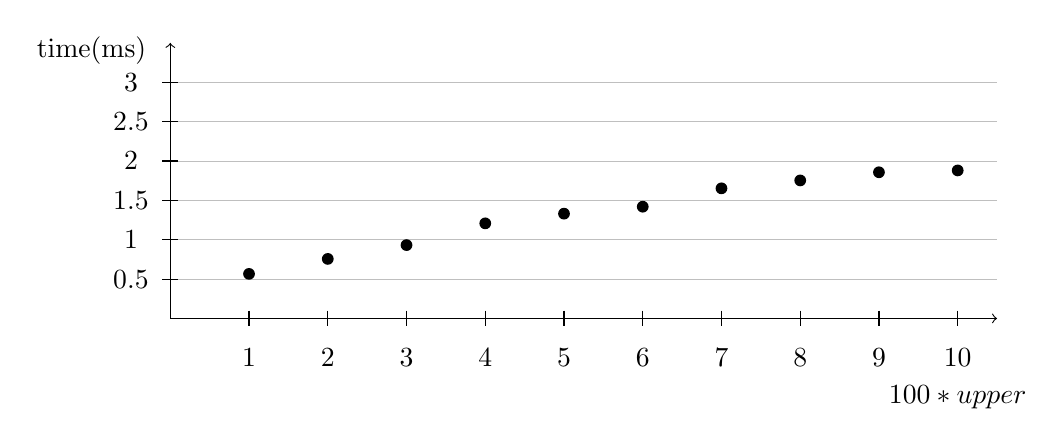
\begin{tikzpicture}
				%time axis
				\draw[->] (0,0) -- (0,3.5);
				\node at (-1, 3.4){time(ms)};
%				\foreach \y in {0.25, 0.5, ..., 3}{
%					\draw(-0.05, \y)--(0.05, \y);
%				}
				\foreach \y in {0.5, 1, 1.5, 2, 2.5, 3}{
					\draw[very thin, lightgray] (0, \y)--(10.5, \y);
					\draw(-0.1, \y)--(0.1, \y);
					\node at (-0.5, \y){\y};
					
				}
				
				\draw[->] (0,0) -- (10.5, 0);
				\node at (10, -1){$100*upper$};
				\foreach \x in {1, 2, ..., 10}{
					\draw(\x, 0.1)--(\x, -0.1);
					\node at (\x, -0.5){${\x}$};
				}
				\node at (1, 0.5661) [circle,fill,inner sep=1.5pt]{};
				\node at (2, 0.7561) [circle,fill,inner sep=1.5pt]{};
				\node at (3, 0.9318) [circle,fill,inner sep=1.5pt]{};
				\node at (4, 1.2077) [circle,fill,inner sep=1.5pt]{};
				\node at (5, 1.3308) [circle,fill,inner sep=1.5pt]{};
				\node at (6, 1.4193) [circle,fill,inner sep=1.5pt]{};
				\node at (7, 1.6525) [circle,fill,inner sep=1.5pt]{};
				\node at (8, 1.7528) [circle,fill,inner sep=1.5pt]{};
				\node at (9, 1.8565) [circle,fill,inner sep=1.5pt]{};
				\node at (10, 1.8798) [circle,fill,inner sep=1.5pt]{};
			\end{tikzpicture}
		\centering
		\caption{Average run times of the \textit{DelayConstraint} with event distances of $2^0=1$}
		\label{fig:runtimeDelay1}
	\end{figure}
	\begin{figure}
		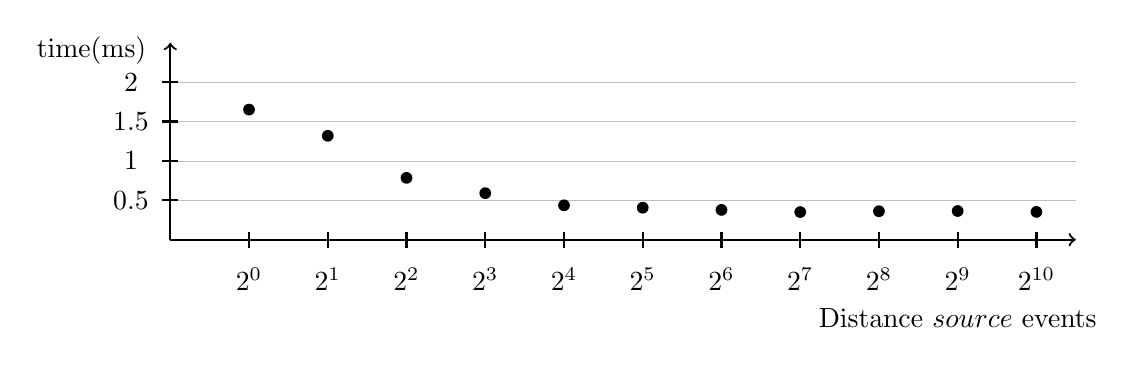
\begin{tikzpicture}[thick]
			%time axis
			\draw[->] (0,0) -- (0,2.5);
			\node at (-1, 2.4){time(ms)};
%			\foreach \y in {0.25, 0.5, ..., 2}{
%				\draw(-0.05, \y)--(0.05, \y);
%			}
			\foreach \y in {0.5, 1, 1.5, 2}{
				\draw[very thin, lightgray] (0, \y)--(11.5, \y);
				\draw(-0.1, \y)--(0.1, \y);
				\node at (-0.5, \y){\y};
				
			}
			
			\draw[->] (0,0) -- (11.5, 0);
			\node at (10, -1){Distance $source$ events};
			\foreach \x in {0, 1, 2, ..., 10}{
				\draw(\x+1, 0.1)--(\x+1, -0.1);
				\node at (\x+1, -0.5){$2^{\x}$};
			}
			\node at (1, 1.6525) [circle,fill,inner sep=1.5pt]{};
			\node at (2, 1.3198) [circle,fill,inner sep=1.5pt]{};
			\node at (3, 0.7854) [circle,fill,inner sep=1.5pt]{};
			\node at (4, 0.591) [circle,fill,inner sep=1.5pt]{};
			\node at (5, 0.4368) [circle,fill,inner sep=1.5pt]{};
			\node at (6, 0.4066) [circle,fill,inner sep=1.5pt]{};
			\node at (7, 0.3786) [circle,fill,inner sep=1.5pt]{};
			\node at (8, 0.3511) [circle,fill,inner sep=1.5pt]{};
			\node at (9, 0.3617) [circle,fill,inner sep=1.5pt]{};
			\node at (10, 0.3646) [circle,fill,inner sep=1.5pt]{};
			\node at (11, 0.3532) [circle,fill,inner sep=1.5pt]{};
		\end{tikzpicture}
		\centering
		\caption{Average run times of the \textit{DelayConstraint} with the parameters $lower = upper = 700$}
		\label{fig:runtimeDelay2}
	\end{figure}


\subsubsection{StrongDelayConstraint}
	The traces for the evaluation of the \textit{StrongDelayConstraint} were generated with the same parameters as for the previous constraint. In figure~\ref{fig:runtimeStrongDelay1} the average run times with fixed $source$ event distances is shown. The results are nearly constant. Figure~\ref{fig:runtimeStrongDelay2} shows the average run times for traces, where $lower$ and $upper$ is fixed to 700 and the distance between subsequent $source$ is varying. It can be seen, that the run times for the traces is separated into two areas, one cluster containing the traces with a $source$ event distance of $2^0, 2^1$ and $2^2$ and one containing the other traces. These clusters can be seen at all different values for $lower$ and $upper$, but they are not always containing the traces with the same distance between the $source$ events. The reason for this behaviour is, that in some traces $source$ and $target$ events occur in the same timestamps and in some traces, all timestamps only have at most one timestamp. Because processing two events takes more time than processing one event, the average run time per input timestamp is higher, when more events are processed in less timestamps.\\
	When the distance between the $source$ events is 1, the parameters $lower$ and $upper$ are set to 700 and 10.000 events are generated, 1.400 timestamps consists of one timestamp and 4.300 timestamp consists of two events. At a distance of 2, 700 timestamps have one event and 4650 timestamps contain 2 events. When the distance is 4, 350 events occur singly and the others occur in 4825 timestamps. In the traces with a $source$ event distance of 8, 16, 32, 64, 128, 256, 512 and 1024, all events occur in individual timestamps, so the run times of them is lower.
	\begin{proof}
		Let $lower=upper=700$ be the distance between $source$ events and their associated $target$ event.\\
		Let $s\in\mathbb{N}_0$ be the first timestamp with an $source$ event in the trace.\\
		Let $dist\in\mathbb{N}$ be the distance between subsequent $source$ events.\\
		The placement of all $source$ events is given by: $s+x*dist$ with $x\in\mathbb N$\\
		The placement of all $target$ events is given by: $s+y*dist + 700$ with $y\in\mathbb N, y<x$\\
		All placements of $source$ and $target$ events, which occur in common timestamps, fulfilled the equation:\\
		\begin{align}
			s+x*dist&=s+y*dist+upper\\
			x*dist&=y*dist+upper\\
			x&= y + \frac{upper}{dist}
		\end{align}
		Because there is no integer solution for $x$ and $y$ for $dist\in{8,16,32,64,128,256,512,1024}$, all events occur in individual timestamps, when $upper$ is set to 700.
	\end{proof}
	\begin{figure}
		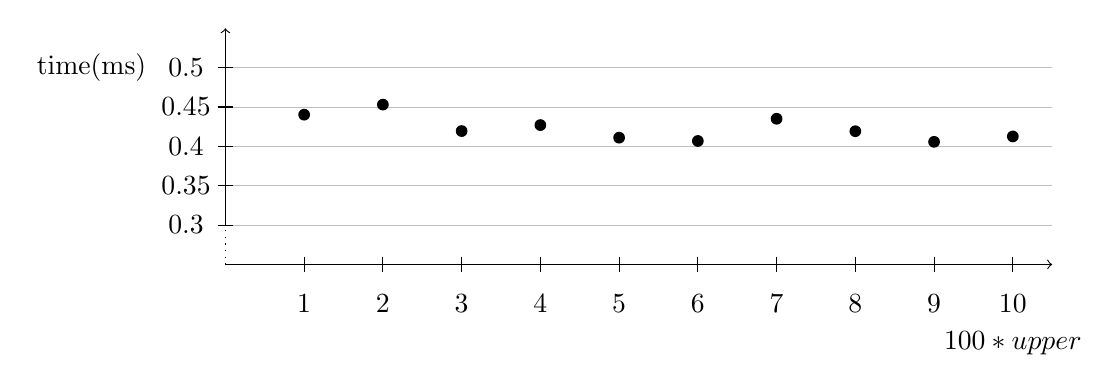
\begin{tikzpicture}[yscale=10]
			%time axis
			\draw[->] (0,0.3) -- (0,0.55);
			\draw[dotted](0,0.25)--(0,0.3);
			\node at (-1.7, 0.5){time(ms)};
			
			\foreach \y in {0.3, 0.35, 0.4, 0.45, 0.5}{
				\draw[very thin, lightgray] (0, \y)--(10.5, \y);
				\draw(-0.1, \y)--(0.1, \y);
				\node at (-0.5, \y){\y};
				
			}
			
			\draw[->] (0,0.25) -- (10.5, 0.25);
			\node at (10, 0.15){$100*upper$};
			\foreach \x in {1, 2, ..., 10}{
				\draw(\x, 0.26)--(\x, 0.24);
				\node at (\x, 0.2){${\x}$};
			}
			\node at (1, 0.4402) [circle,fill,inner sep=1.5pt]{};
			\node at (2, 0.453) [circle,fill,inner sep=1.5pt]{};
			\node at (3, 0.4194) [circle,fill,inner sep=1.5pt]{};
			\node at (4, 0.427) [circle,fill,inner sep=1.5pt]{};
			\node at (5, 0.411) [circle,fill,inner sep=1.5pt]{};
			\node at (6, 0.4068) [circle,fill,inner sep=1.5pt]{};
			\node at (7, 0.435) [circle,fill,inner sep=1.5pt]{};
			\node at (8, 0.4192) [circle,fill,inner sep=1.5pt]{};
			\node at (9, 0.4057) [circle,fill,inner sep=1.5pt]{};
			\node at (10, 0.4126) [circle,fill,inner sep=1.5pt]{};
		\end{tikzpicture}
		\centering
		\caption{Average run times of the \textit{StrongDelayConstraint} with event distances of $2^0=1$}
		\label{fig:runtimeStrongDelay1}
	\end{figure}
\begin{figure}
	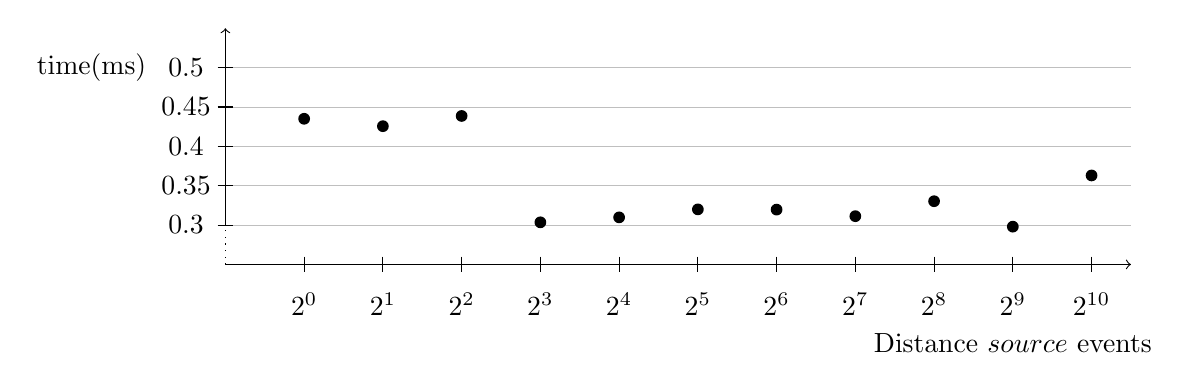
\begin{tikzpicture}[yscale=10]
			%time axis
			\draw[->] (0,0.3) -- (0,0.55);
			\draw[dotted](0,0.25)--(0,0.3);
			\node at (-1.7, 0.5){time(ms)};
			
			\foreach \y in {0.3, 0.35, 0.4, 0.45, 0.5}{
				\draw[very thin, lightgray] (0, \y)--(11.5, \y);
				\draw(-0.1, \y)--(0.1, \y);
				\node at (-0.5, \y){\y};
				
			}
			
			\draw[->] (0,0.25) -- (11.5, 0.25);
			\node at (10, 0.15){Distance $source$ events};
			\foreach \x in {0, 1, 2, ..., 10}{
				\draw(\x+1, 0.26)--(\x+1, 0.24);
				\node at (\x+1, 0.2){$2^{\x}$};
			}
			\node at (1, 0.435) [circle,fill,inner sep=1.5pt]{};
			\node at (2, 0.4256) [circle,fill,inner sep=1.5pt]{};
			\node at (3, 0.43858) [circle,fill,inner sep=1.5pt]{};
			\node at (4, 0.3035) [circle,fill,inner sep=1.5pt]{};
			\node at (5, 0.3098) [circle,fill,inner sep=1.5pt]{};
			\node at (6, 0.31994) [circle,fill,inner sep=1.5pt]{};
			\node at (7, 0.31964) [circle,fill,inner sep=1.5pt]{};
			\node at (8, 0.3113) [circle,fill,inner sep=1.5pt]{};
			\node at (9, 0.3303) [circle,fill,inner sep=1.5pt]{};
			\node at (10, 0.298) [circle,fill,inner sep=1.5pt]{};
			\node at (11, 0.363) [circle,fill,inner sep=1.5pt]{};
		\end{tikzpicture}
	\centering
	\caption{Average run times of the \textit{StrongDelayConstraint} with the parameters $lower = upper = 700$}
	\label{fig:runtimeStrongDelay2}
\end{figure}


\subsubsection{RepeatConstraint}
	The \textit{RepeatConstraint} was evaluated with 100 Traces of 10.000 events. The traces were created with the attributes $span\in\{1,300,600,900\}$, $lower=\{5000,6000,7000,8000,9000\}$ and $upper=lower+x$, $x\in{1000,2000,3000,4000}$.  Figure~\ref{fig:RepeatConstraintRuntime3} shows the average run time with a fixed $span$ and $lower$ parameter and a variable value for $upper$. It can be seen, that the run times are nearly constant, which matches with the analysis of the implementation.\\ Figure~\ref{fig:RepeatConstraintRuntime1} and \ref{fig:RepeatConstraintRuntime2} show the average run time of the \textit{RepeatConstraint} monitor with the parameters $lower=5000$(7000), $upper=7000$(10000). By the analysis of the implementation, a runtime that is linear dependent on $span$ was expected, which can be slightly seen in the results. The increase is not much larger than the deviations between individual measures, but can be seen by nearly all runs with different values for $lower$ and $upper$. 
%	An explanation for this fairly small increase is that the linear growth of the run time is proclaimed by the use of $nLastTime$ macro, which is defined as\\[10pt]
%		\textcolor{red}{def} nLastTime[\textcolor{blue}{A}](e: \textcolor{brown}{Events}[\textcolor{blue}{A}], n: \textcolor{blue}{Int}): \textcolor{brown}{Events}[\textcolor{blue}{Int}] :=\\ \hbox{}
%		\quad\textcolor{red}{static if} (n <= 0) \textcolor{red}{then}\\ \hbox{}
%		\quad\quad time(e)\\ \hbox{}
%		\quad \textcolor{red}{else}\\ \hbox{}
%		\quad\quad last(nLastTime(e, n-1), e)\\[10pt]
%	The parameter $span$ is used as $span$ in this macro, so the macro is called with 1, 300, 600 or 900 in each input timestamp. 

	
\begin{figure}
	\centering
	\begin{minipage}{0.45\textwidth}
		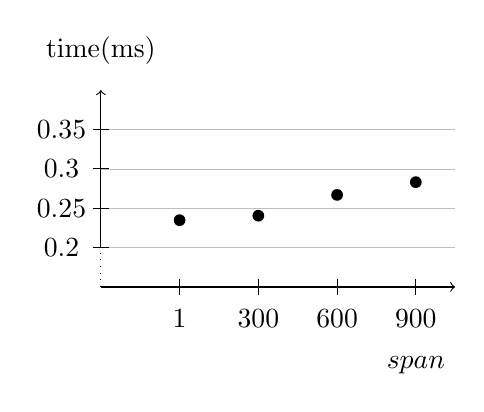
\begin{tikzpicture}[yscale=10]
			%time axis
			\draw[->] (0,0.2) -- (0,0.4);
			\draw[dotted] (0, 0.15) -- (0,0.2);
			\node at (0, 0.45){time(ms)};
			
			\foreach \y in {0.2, 0.25, 0.3, 0.35}{
				\draw[very thin, lightgray] (0, \y)--(4.5, \y);
				\draw(-0.1, \y)--(0.1, \y);
				\node at (-0.5, \y){\y};
				
			}
			
			\draw[->] (0,0.15) -- (4.5, 0.15);
			\node at (4, 0.05){$span$};
			\foreach \x in {0, 1, 2, ..., 3}{
				\draw(\x+1, 0.16)--(\x+1, 0.14);
			}
			\node at (1, 0.11){$1$};
			\node at (2, 0.11){$300$};
			\node at (3, 0.11){$600$};
			\node at (4, 0.11){$900$};
			
			%\draw (1, 0.2491) -- (2, 0.2743) -- (3, 0.25835) -- (4, 0.2737);
			
			\node at (1, 0.2348) [circle,fill,inner sep=1.5pt]{};
			\node at (2, 0.2405) [circle,fill,inner sep=1.5pt]{};
			\node at (3, 0.2669) [circle,fill,inner sep=1.5pt]{};
			\node at (4, 0.2831) [circle,fill,inner sep=1.5pt]{};
		\end{tikzpicture}
		\centering
		\caption{Average run times of the\\ \textit{RepeatConstraint} with the\\ parameters $lower = 5000, upper = 6000$}
		\label{fig:RepeatConstraintRuntime1}
	\end{minipage}\hfill
	\begin{minipage}{0.45\textwidth}
		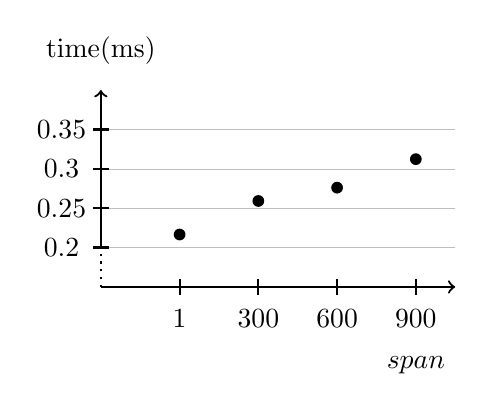
\begin{tikzpicture}[thick, yscale=10]
			%time axis
			\draw[->] (0,0.2) -- (0,0.4);
			\draw[dotted] (0, 0.15) -- (0,0.2);
			\node at (0, 0.45){time(ms)};
			
			\foreach \y in {0.2, 0.25, 0.3, 0.35}{
				\draw[very thin, lightgray] (0, \y)--(4.5, \y);
				\draw(-0.1, \y)--(0.1, \y);
				\node at (-0.5, \y){\y};
				
			}
			
			\draw[->] (0,0.15) -- (4.5, 0.15);
			\node at (4, 0.05){$span$};
			\foreach \x in {0, 1, 2, ..., 3}{
				\draw(\x+1, 0.16)--(\x+1, 0.14);
				%\node at (\x+1, -0.05){$2^{\x}$};
			}
			\node at (1, 0.11){$1$};
			\node at (2, 0.11){$300$};
			\node at (3, 0.11){$600$};
			\node at (4, 0.11){$900$};
			\node at (1, 0.2166) [circle,fill,inner sep=1.5pt]{};
			\node at (2, 0.2592) [circle,fill,inner sep=1.5pt]{};
			\node at (3, 0.2761) [circle,fill,inner sep=1.5pt]{};
			\node at (4, 0.3123) [circle,fill,inner sep=1.5pt]{};
		\end{tikzpicture}
		\centering
		\caption{Average run times of the\\ \textit{RepeatConstraint} with the parameters\\ $lower = 7000, upper = 10000$}
		\label{fig:RepeatConstraintRuntime2}
	\end{minipage}
\end{figure}

\begin{figure}
	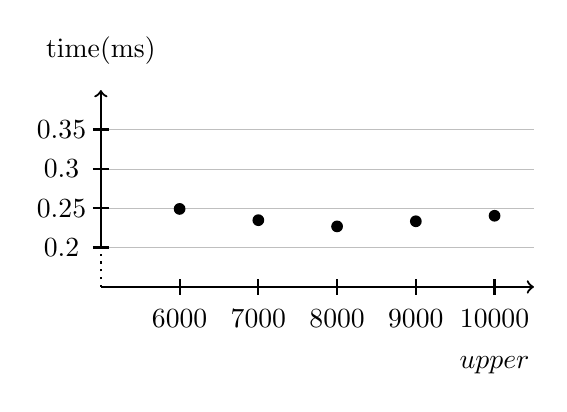
\begin{tikzpicture}[thick, yscale=10]
	%time axis
	\draw[->] (0,0.2) -- (0,0.4);
	\draw[dotted] (0, 0.15) -- (0,0.2);
	\node at (0, 0.45){time(ms)};
	
	\foreach \y in {0.2, 0.25, 0.3, 0.35}{
		\draw[very thin, lightgray] (0, \y)--(5.5, \y);
		\draw(-0.1, \y)--(0.1, \y);
		\node at (-0.5, \y){\y};
		
	}
	
	\draw[->] (0,0.15) -- (5.5, 0.15);
	\node at (5, 0.05){$upper$};
	\foreach \x in {0, 1, 2, ..., 4}{
		\draw(\x+1, 0.16)--(\x+1, 0.14);
		%\node at (\x+1, -0.05){$2^{\x}$};
	}
	\node at (1, 0.11){$6000$};
	\node at (2, 0.11){$7000$};
	\node at (3, 0.11){$8000$};
	\node at (4, 0.11){$9000$};
	\node at (5, 0.11){$10000$};
	
	
	\node at (1, 0.2491) [circle,fill,inner sep=1.5pt]{};
	\node at (2, 0.2348) [circle,fill,inner sep=1.5pt]{};
	\node at (3, 0.2269) [circle,fill,inner sep=1.5pt]{};
	\node at (4, 0.2334) [circle,fill,inner sep=1.5pt]{};
	\node at (5, 0.2404) [circle,fill,inner sep=1.5pt]{};
	\end{tikzpicture}
	\centering
	\caption{Average run times of the \textit{RepeatConstraint} with the parameters $span = 250,  lower = 500$}
	\label{fig:RepeatConstraintRuntime3}
\end{figure}

\subsubsection{RepetitionConstraint}
	The traces for this constraint was created with the parameters $span\in\{1,100,250,500\}$, $lower=\{500,600,700,800,900\}$ $upper=lower+x$, $x\in{400,500,600,700,800}$ and $jitter=\frac{lower}{2}$. The run time per input timestamp was between 0.16ms and 50.38ms, averaging around 0.31ms. Figure~\ref{fig:RepetitionConstraintRuntime1} and \ref{fig:RepetitionConstraintRuntime2} are showing the average run times of the monitor with the parameters $lower=500$(700) and $upper=900$(1100) with different values of the $span$ parameter. Figure~\ref{fig:RepetitionConstraintRuntime3} shows the average run time in dependency of the $upper$ parameter. Like expected in the analysis, the parameters did not an influence to the run times and the run times are nearly constant.
\begin{figure}
	\centering
	\begin{minipage}{0.45\textwidth}
		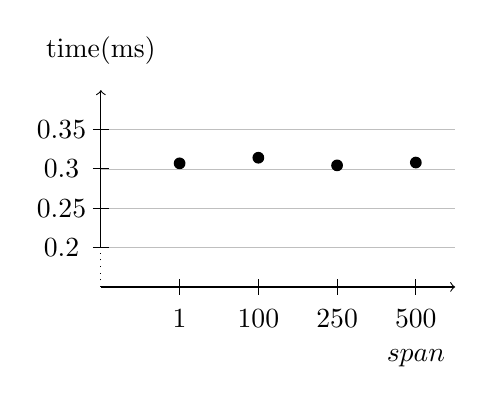
\begin{tikzpicture}[yscale=10]
		%time axis
		\draw[->] (0,0.2) -- (0,0.4);
		\draw[dotted] (0, 0.15) -- (0,0.2);
		\node at (0, 0.45){time(ms)};
			
		\foreach \y in {0.2, 0.25, 0.3, 0.35}{
			\draw[very thin, lightgray] (0, \y)--(4.5, \y);
			\draw(-0.1, \y)--(0.1, \y);
			\node at (-0.5, \y){\y};
		
		}
		
		\draw[->] (0,0.15) -- (4.5, 0.15);
		\node at (4, 0.06){$span$};
		\foreach \x in {0, 1, 2, ..., 3}{
			\draw(\x+1, 0.16)--(\x+1, 0.14);
		}
		\node at (1, 0.11){$1$};
		\node at (2, 0.11){$100$};
		\node at (3, 0.11){$250$};
		\node at (4, 0.11){$500$};
		\node at (1, 0.30697) [circle,fill,inner sep=1.5pt]{};
		\node at (2, 0.3141) [circle,fill,inner sep=1.5pt]{};
		\node at (3, 0.3044) [circle,fill,inner sep=1.5pt]{};
		\node at (4, 0.3080) [circle,fill,inner sep=1.5pt]{};
		\end{tikzpicture}
		\centering
		\caption{Average run times of the\\ \textit{RepetitionConstraint} with the\\ parameters $lower = 500, upper = 900$}
		\label{fig:RepetitionConstraintRuntime1}
	\end{minipage}\hfill
	\begin{minipage}{0.45\textwidth}
		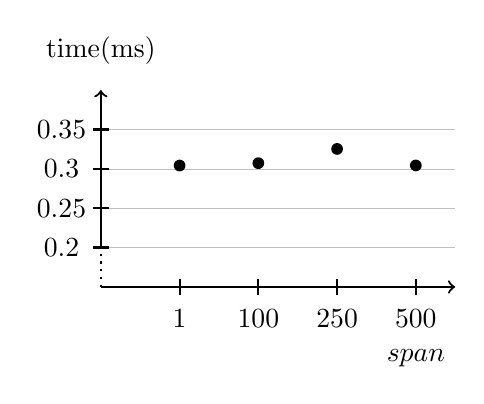
\begin{tikzpicture}[thick, yscale=10]
		%time axis
		\draw[->] (0,0.2) -- (0,0.4);
		\draw[dotted] (0, 0.15) -- (0,0.2);
		\node at (0, 0.45){time(ms)};
		
		\foreach \y in {0.2, 0.25, 0.3, 0.35}{
			\draw[very thin, lightgray] (0, \y)--(4.5, \y);
			\draw(-0.1, \y)--(0.1, \y);
			\node at (-0.5, \y){\y};
		
		}
		
		\draw[->] (0,0.15) -- (4.5, 0.15);
		\node at (4, 0.06){$span$};
		\foreach \x in {0, 1, 2, ..., 3}{
			\draw(\x+1, 0.16)--(\x+1, 0.14);
		}
		\node at (1, 0.11){$1$};
		\node at (2, 0.11){$100$};
		\node at (3, 0.11){$250$};
		\node at (4, 0.11){$500$};
		\node at (1, 0.3042) [circle,fill,inner sep=1.5pt]{};
		\node at (2, 0.3072) [circle,fill,inner sep=1.5pt]{};
		\node at (3, 0.3253) [circle,fill,inner sep=1.5pt]{};
		\node at (4, 0.3043) [circle,fill,inner sep=1.5pt]{};
		\end{tikzpicture}
		\centering
		\caption{Average run times of the\\ \textit{RepetitionConstraint} with the parameters\\ $lower = 700, upper = 1100$}
		\label{fig:RepetitionConstraintRuntime2}
	\end{minipage}
\end{figure}
	
\begin{figure}
	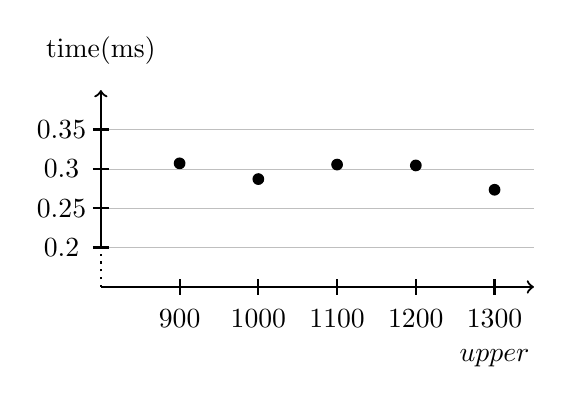
\begin{tikzpicture}[thick, yscale=10]
	%time axis
	\draw[->] (0,0.2) -- (0,0.4);
	\draw[dotted] (0, 0.15) -- (0,0.2);
	\node at (0, 0.45){time(ms)};
	
	\foreach \y in {0.2, 0.25, 0.3, 0.35}{
		\draw[very thin, lightgray] (0, \y)--(5.5, \y);
		\draw(-0.1, \y)--(0.1, \y);
		\node at (-0.5, \y){\y};
		
	}
	
	\draw[->] (0,0.15) -- (5.5, 0.15);
	\node at (5, 0.06){$upper$};
	\foreach \x in {0, 1, 2, ..., 4}{
		\draw(\x+1, 0.16)--(\x+1, 0.14);
		%\node at (\x+1, -0.05){$2^{\x}$};
	}
	\node at (1, 0.11){$900$};
	\node at (2, 0.11){$1000$};
	\node at (3, 0.11){$1100$};
	\node at (4, 0.11){$1200$};
	\node at (5, 0.11){$1300$};
	
	
	\node at (1, 0.30697) [circle,fill,inner sep=1.5pt]{};
	\node at (2, 0.28699) [circle,fill,inner sep=1.5pt]{};
	\node at (3, 0.30542) [circle,fill,inner sep=1.5pt]{};
	\node at (4, 0.3043) [circle,fill,inner sep=1.5pt]{};
	\node at (5, 0.27342) [circle,fill,inner sep=1.5pt]{};
	\end{tikzpicture}
	\centering
	\caption{Average run times of the \textit{RepetitionConstraint} with the parameters $span = 1,  lower = 500$}
	\label{fig:RepetitionConstraintRuntime3}
\end{figure}
	
	
\subsubsection{SynchronizationConstraint}
Figure~\ref{fig:SynchronizationConstraintConstraintRunTime1} shows the average run times of the \textit{SynchronizationConstraint} monitor, which was checking traces with three event streams with two events per synchronization cluster in each stream. The synchronization clusters were 200 timestamps apart, so they do not overlap. The run times were nearly constant, which was expected for these parameters, because at most 3 (the number of input streams) events were stored and considered in each input time stamp.\\
Figure~\ref{fig:SynchronizationConstraintConstraintRunTime2} shows the average run times of the monitor with traces of three streams, a $tolerance$ value of 91 and a distance between clusters of 182. So again, the clusters were not overlapping. It can be seen, that the run times grow linear when increasing the number of events in each cluster. This matches with the expectation, because the more events occur in an interval of the length $tolerance$, the more events need to be stored and considered in each input timestamp.
\begin{figure}
	\centering
	\begin{minipage}{0.45\textwidth}
		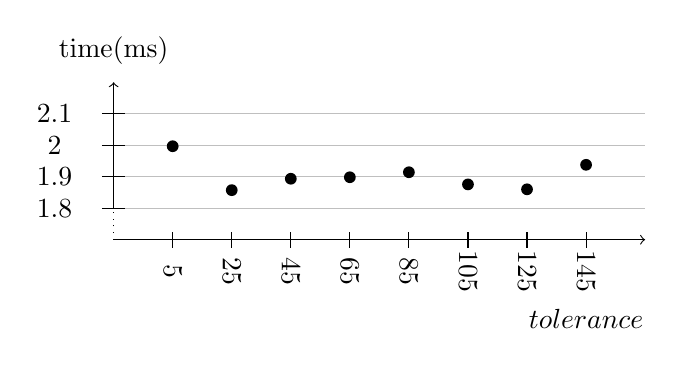
\begin{tikzpicture}[yscale=4, xscale=1.5]
		%time axis
		\draw[->] (0,1.8) -- (0,2.2);
		\draw[dotted] (0, 1.7) -- (0,1.8);
		\node at (0, 2.3){time(ms)};
		
		\foreach \y in {1.8,1.9,2, 2.1}{
			\draw[very thin, lightgray] (0, \y)--(4.5, \y);
			\draw(-0.1, \y)--(0.1, \y);
			\node at (-0.5, \y){\y};
			
		}
		
		\draw[->] (0,1.7) -- (4.5, 1.7);
		\node at (4, 1.45){$tolerance$};
		\foreach \x in {0.5, 1, 1.5, 2, 2.5, 3, 3.5, 4}{
			\draw(\x, 1.675)--(\x, 1.725);
		}
		\node[rotate=270] at (0.5, 1.6){$5$};
		\node[rotate=270] at (1, 1.6){$25$};
		\node[rotate=270] at (1.5, 1.6){$45$};
		\node[rotate=270] at (2, 1.6){$65$};
		\node[rotate=270] at (2.5, 1.6){$85$};
		\node[rotate=270] at (3, 1.6){$105$};
		\node[rotate=270] at (3.5, 1.6){$125$};
		\node[rotate=270] at (4, 1.6){$145$};
		\node at (0.5, 1.9968) [circle,fill,inner sep=1.5pt]{};
		\node at (1, 1.8573) [circle,fill,inner sep=1.5pt]{};
		\node at (1.5, 1.8936) [circle,fill,inner sep=1.5pt]{};
		\node at (2, 1.8983) [circle,fill,inner sep=1.5pt]{};
		\node at (2.5, 1.9142) [circle,fill,inner sep=1.5pt]{};
		\node at (3, 1.8756) [circle,fill,inner sep=1.5pt]{};
		\node at (3.5, 1.86) [circle,fill,inner sep=1.5pt]{};
		\node at (4, 1.9378) [circle,fill,inner sep=1.5pt]{};
		\end{tikzpicture}
		\centering
		\caption{Average run times of the\\ \textit{SynchronizationConstraint} with three event\\ streams and two events per cluster and stream\\ and a cluster distance of 200}
		\label{fig:SynchronizationConstraintConstraintRunTime1}
	\end{minipage}\hfill
	\begin{minipage}{0.45\textwidth}
		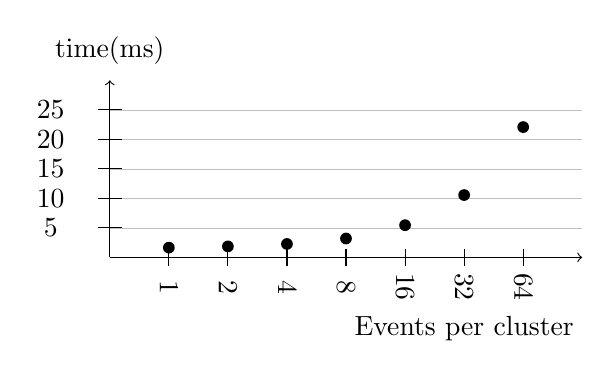
\begin{tikzpicture}[yscale=0.075, xscale=1.5]
			%time axis
			\draw[->] (0,0) -- (0,30);
			\node at (0, 35){time(ms)};
			
			\foreach \y in {5, 10, ..., 25}{
				\draw[very thin, lightgray] (0, \y)--(4, \y);
				\draw(-0.1, \y)--(0.1, \y);
				\node at (-0.5, \y){\y};
				
			}
			
			\draw[->] (0,0) -- (4,0);
			\node at (3, -12){Events per cluster};
			\foreach \x in {0.5, 1, 1.5, 2, 2.5, 3, 3.5}{
				\draw(\x, 1.5)--(\x, -1.5);
			}
			\node[rotate=270] at (0.5, -5){$1$};
			\node[rotate=270] at (1, -5){$2$};
			\node[rotate=270] at (1.5, -5){$4$};
			\node[rotate=270] at (2, -5){$8$};
			\node[rotate=270] at (2.5, -5){$16$};
			\node[rotate=270] at (3, -5){$32$};
			\node[rotate=270] at (3.5, -5){$64$};
			\node at (0.5, 1.6568) [circle,fill,inner sep=1.5pt]{};
			\node at (1, 1.8676) [circle,fill,inner sep=1.5pt]{};
			\node at (1.5, 2.2772) [circle,fill,inner sep=1.5pt]{};
			\node at (2, 3.2023) [circle,fill,inner sep=1.5pt]{};
			\node at (2.5, 5.4592) [circle,fill,inner sep=1.5pt]{};
			\node at (3, 10.5615) [circle,fill,inner sep=1.5pt]{};
			\node at (3.5, 22.0735) [circle,fill,inner sep=1.5pt]{};
		\end{tikzpicture}
		\centering
		\caption{Average run times of the\\ \textit{SynchronizationConstraint} with three event streams,\\ $tolerance=91$ and a cluster distance of $182$ }
		\label{fig:SynchronizationConstraintConstraintRunTime2}
	\end{minipage}
\end{figure}


\subsubsection{StrongSynchronizationConstraint}
	Figure~\ref{fig:StrongSynchronizationConstraintConstraintRunTime1} shows the average run time of the monitor with the parameters $tolerance = 37$ and a cluster distance of 2, so that 19 clusters are overlapping. It can be seen, that the run time increases, when more input streams are used. In Figure~\ref{fig:StrongSynchronizationConstraintConstraintRunTime2}, a fixed number of input streams was used and the cluster distance was 2, like before. Again, an increase in the run times can be seen. This matches with the expectations of the analysis, in which the run time was said to be in $\mathcal{O}(|event| * tolerance)$.

\begin{figure}
	\centering
	\begin{minipage}{0.45\textwidth}
%		\begin{tikzpicture}[yscale=20]
%		%time axis
%		\draw[->] (0,0.775) -- (0,0.875);
%		\draw[dotted] (0, 0.75) -- (0,0.775);
%		\node at (0, 0.9){time(ms)};
%		
%		\foreach \y in {0.775, 0.8, 0.825, 0.85}{
%			\draw[very thin, lightgray] (0, \y)--(4.5, \y);
%			\draw(-0.1, \y)--(0.1, \y);
%			\node at (-1, \y){\y};
%			
%		}
%		
%		\draw[->] (0,0.75) -- (4.5, 0.75);
%		\node at (3, 0.7){Cluster Distance};
%		\foreach \x in { 1, 2, 3, 4}{
%			\draw(\x, 0.745)--(\x, 0.755);
%		}
%		\node[rotate=270] at (1, 0.7255){$2$};
%		\node[rotate=270] at (2, 0.7255){$8$};
%		\node[rotate=270] at (3, 0.7255){$32$};
%		\node[rotate=270] at (4, 0.7255){$128$};
%		\node at (1, 0.7828) [circle,fill,inner sep=1.5pt]{};
%		\node at (2, 0.8206) [circle,fill,inner sep=1.5pt]{};
%		\node at (3, 0.7894) [circle,fill,inner sep=1.5pt]{};
%		\node at (4, 0.8319) [circle,fill,inner sep=1.5pt]{};
%		\end{tikzpicture}
%		\centering
%		\caption{Average run times of the\\ \textit{StrongSynchronizationConstraint} with two\\ event streams and $tolerance=1$}
%		\label{fig:StrongSynchronizationConstraintConstraintRunTime1}
		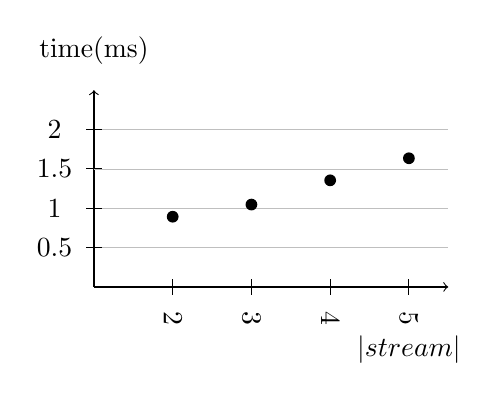
\begin{tikzpicture}
		%time axis
		\draw[->] (0,0) -- (0,2.5);
		\node at (0, 3){time(ms)};
		
		\foreach \y in {0.5, 1, 1.5, 2}{
			\draw[very thin, lightgray] (0, \y)--(4.5, \y);
			\draw(-0.1, \y)--(0.1, \y);
			\node at (-0.5, \y){\y};
			
		}
		
		\draw[->] (0,0) -- (4.5, 0);
		\node at (4, -0.8){$|stream|$};
		\foreach \x in {1,2,3,4}{
			\draw(\x, 0.1)--(\x, -0.1);
		}
		\node[rotate=270] at (1, -0.4){$2$};
		\node[rotate=270] at (2, -0.4){$3$};
		\node[rotate=270] at (3, -0.4){$4$};
		\node[rotate=270] at (4, -0.4){$5$};
		\node at (1, 0.8921) [circle,fill,inner sep=1.5pt]{};
		\node at (2, 1.0464) [circle,fill,inner sep=1.5pt]{};
		\node at (3, 1.3541) [circle,fill,inner sep=1.5pt]{};
		\node at (4, 1.6345) [circle,fill,inner sep=1.5pt]{};
		\end{tikzpicture}
		\centering
		\caption{Average run times of the\\ \textit{StrongSynchronizationConstraint} with\\ $tolerance=37$ and a cluster distance of 2}
		\label{fig:StrongSynchronizationConstraintConstraintRunTime1}
	\end{minipage}\hfill
	\begin{minipage}{0.45\textwidth}
		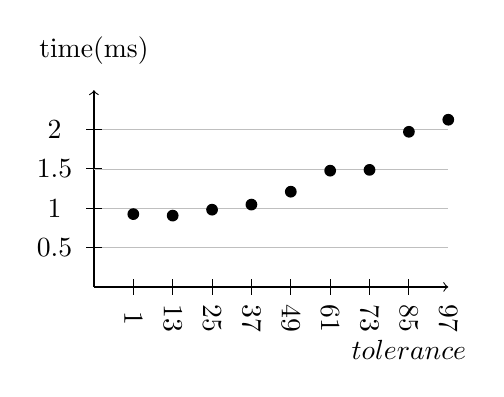
\begin{tikzpicture}
		%time axis
		\draw[->] (0,0) -- (0,2.5);
		\node at (0, 3){time(ms)};
		
		\foreach \y in {0.5, 1, 1.5, 2}{
			\draw[very thin, lightgray] (0, \y)--(4.5, \y);
			\draw(-0.1, \y)--(0.1, \y);
			\node at (-0.5, \y){\y};
			
		}
		
		\draw[->] (0,0) -- (4.5, 0);
		\node at (4, -0.8){$tolerance$};
		\foreach \x in {0.5, 1, 1.5, 2, 2.5, 3, 3.5, 4}{
			\draw(\x, 0.1)--(\x, -0.1);
		}
		\node[rotate=270] at (0.5, -0.4){$1$};
		\node[rotate=270] at (1, -0.4){$13$};
		\node[rotate=270] at (1.5, -0.4){$25$};
		\node[rotate=270] at (2, -0.4){$37$};
		\node[rotate=270] at (2.5, -0.4){$49$};
		\node[rotate=270] at (3, -0.4){$61$};
		\node[rotate=270] at (3.5, -0.4){$73$};
		\node[rotate=270] at (4, -0.4){$85$};
		\node[rotate=270] at (4.5, -0.4){$97$};
		\node at (0.5, 0.9252) [circle,fill,inner sep=1.5pt]{};
		\node at (1, 0.9062) [circle,fill,inner sep=1.5pt]{};
		\node at (1.5, 0.9813) [circle,fill,inner sep=1.5pt]{};
		\node at (2, 1.046) [circle,fill,inner sep=1.5pt]{};
		\node at (2.5, 1.2098) [circle,fill,inner sep=1.5pt]{};
		\node at (3, 1.4768) [circle,fill,inner sep=1.5pt]{};
		\node at (3.5, 1.4869) [circle,fill,inner sep=1.5pt]{};
		\node at (4, 1.9705) [circle,fill,inner sep=1.5pt]{};
		\node at (4.5, 2.1237) [circle,fill,inner sep=1.5pt]{};
		\end{tikzpicture}
		\centering
		\caption{Average run times of the\\ \textit{StrongSynchronizationConstraint} with three\\ event streams and a cluster distance of 2}
		\label{fig:StrongSynchronizationConstraintConstraintRunTime2}
	\end{minipage}
\end{figure}




\subsubsection{ExecutionTimeConstraint}
	The run time evaluation of the \textit{ExecutionTimeConstraint} monitor was done by traces, which fulfill the constraint the parameters $lower\in\{100,300,500,700,900\}$ and $upper=lower+x$, $x\in\{100,600,1100,1600,2100\}$. For each of combination of these parameters, one trace with 1, 11, 21 and 31 preemptions between the each $start$ and $end$ event were created. The run times were between 0.014ms and 33.6ms with an average of 0.19ms. In figure~\ref{fig:ExecutionTimeConstraintRunTime1} the average run time with fixed $lower$ and $upper$ can be seen. In figure~\ref{fig:ExecutionTimeConstraintRunTime2}, $lower$ and the number of preemptions is fixed. A correlation between the input parameters and the run times can not be observed, which was expected, because the run time is independent from the parameters or the placement of events, like stated in chapter~\ref{chapter-implementation}.
\begin{figure}
	\centering
	\begin{minipage}{0.45\textwidth}
		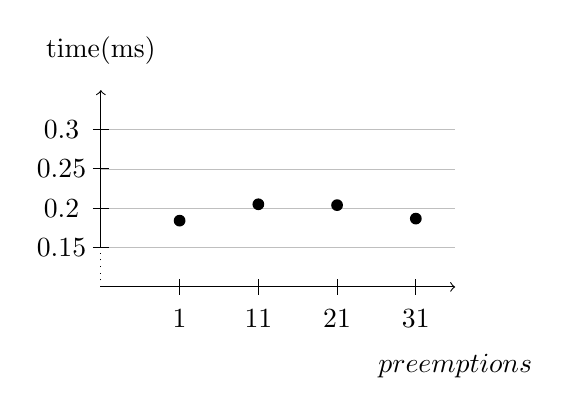
\begin{tikzpicture}[yscale=10]
			%time axis
			\draw[->] (0,0.15) -- (0,0.35);
			\draw[dotted] (0, 0.1) -- (0,0.15);
			\node at (0, 0.4){time(ms)};
			
			\foreach \y in {0.15, 0.2, 0.25, 0.3}{
				\draw[very thin, lightgray] (0, \y)--(4.5, \y);
				\draw(-0.1, \y)--(0.1, \y);
				\node at (-0.5, \y){\y};
				
			}
			
			\draw[->] (0,0.1) -- (4.5, 0.1);
			\node at (4.5, 0.0){$preemptions$};
			\foreach \x in {0, 1, 2, ..., 3}{
				\draw(\x+1, 0.11)--(\x+1, 0.09);
			}
			\node at (1, 0.06){$1$};
			\node at (2, 0.06){$11$};
			\node at (3, 0.06){$21$};
			\node at (4, 0.06){$31$};
			\node at (1, 0.1842) [circle,fill,inner sep=1.5pt]{};
			\node at (2, 0.205) [circle,fill,inner sep=1.5pt]{};
			\node at (3, 0.2039) [circle,fill,inner sep=1.5pt]{};
			\node at (4, 0.1868) [circle,fill,inner sep=1.5pt]{};
		\end{tikzpicture}
		\centering
		\caption{Average run times of the\\ \textit{RepetitionConstraint} with the\\ parameters $lower = 100, upper = 200$}
		\label{fig:ExecutionTimeConstraintRunTime1}
	\end{minipage}\hfill
	\begin{minipage}{0.45\textwidth}
		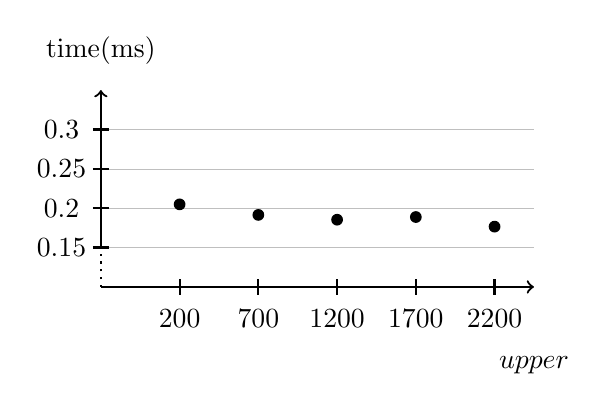
\begin{tikzpicture}[thick, yscale=10]
			%time axis
			\draw[->] (0,0.15) -- (0,0.35);
			\draw[dotted] (0, 0.1) -- (0,0.15);
			\node at (0, 0.4){time(ms)};
			
			\foreach \y in {0.15, 0.2, 0.25, 0.3}{
				\draw[very thin, lightgray] (0, \y)--(5.5, \y);
				\draw(-0.1, \y)--(0.1, \y);
				\node at (-0.5, \y){\y};
				
			}
			
			\draw[->] (0,0.1) -- (5.5, 0.1);
			\node at (5.5, 0.0){$upper$};
			\foreach \x in {0, 1, 2, ..., 3, 4}{
				\draw(\x+1, 0.11)--(\x+1, 0.09);
			}
			\node at (1, 0.06){$200$};
			\node at (2, 0.06){$700$};
			\node at (3, 0.06){$1200$};
			\node at (4, 0.06){$1700$};
			\node at (5, 0.06){$2200$};
			\node at (1, 0.2049) [circle,fill,inner sep=1.5pt]{};
			\node at (2, 0.1915) [circle,fill,inner sep=1.5pt]{};
			\node at (3, 0.1854) [circle,fill,inner sep=1.5pt]{};
			\node at (4, 0.1888) [circle,fill,inner sep=1.5pt]{};
			\node at (5, 0.1766) [circle,fill,inner sep=1.5pt]{};
		\end{tikzpicture}
		\centering
		\caption{Average run times of the\\ \textit{RepetitionConstraint} with the parameters\\ $lower = 100, preemptions = 11$}
		\label{fig:ExecutionTimeConstraintRunTime2}
	\end{minipage}
\end{figure}

\subsubsection{OrderConstraint}
The \textit{OrderConstraint} monitor was evaluated on traces with distances between subsequent $source$ events between 1 and 91 in steps of 10 and maximal distances between the $i^th$ $source$ and $target$ event between 0 and 45 in steps of 5. In traces, where the distance between the $source$ events and their associated $target$ events were 0 or the distance between subsequent $source$ events were 1, the run time is ca. double as large as in the other traces. The reason for this is that the smaller the distance between the $source$ and $target$ events are, the more often two events occur in the same time stamp, which means, that two events must be processed in one timestamp, instead of one, which requires more time.
\begin{figure}
	\centering
	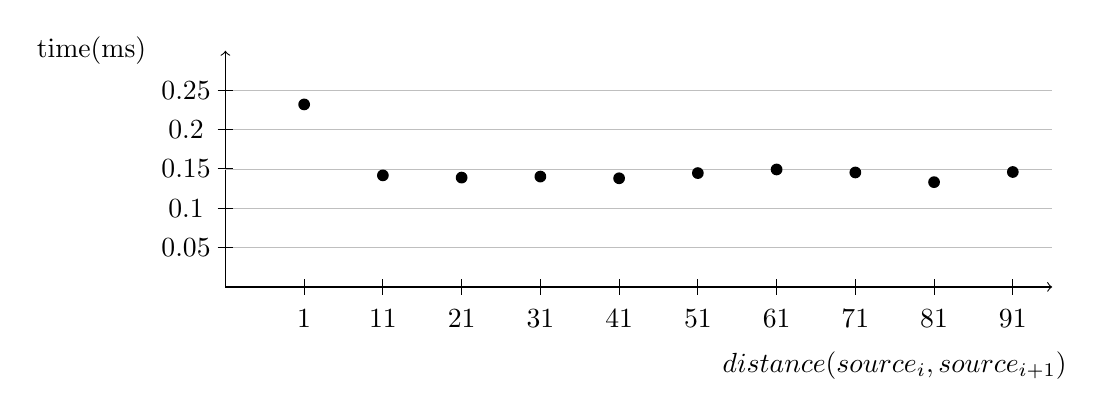
\begin{tikzpicture}[yscale=10]
		%time axis
		\draw[->] (0,0) -- (0,0.3);
		\node at (-1.7, 0.3){time(ms)};
		
		\foreach \y in {0.05, 0.1, 0.15, 0.2, 0.25}{
			\draw[very thin, lightgray] (0, \y)--(10.5, \y);
			\draw(-0.1, \y)--(0.1, \y);
			\node at (-0.5, \y){\y};
			
		}
		
		\draw[->] (0,0) -- (10.5, 0);
		\node at (8.5, -0.1){$distance(source_i, source_{i+1})$};
		\foreach \x in {0, 1, 2, ..., 9}{
			\draw(\x+1, 0.01)--(\x+1, -0.01);
		}
		\node at (1, -0.04){$1$};
		\node at (2, -0.04){$11$};
		\node at (3, -0.04){$21$};
		\node at (4, -0.04){$31$};
		\node at (5, -0.04){$41$};
		\node at (6, -0.04){$51$};
		\node at (7, -0.04){$61$};
		\node at (8, -0.04){$71$};
		\node at (9, -0.04){$81$};
		\node at (10, -0.04){$91$};
		
		\node at (1, 0.2318) [circle,fill,inner sep=1.5pt]{};
		\node at (2, 0.1417) [circle,fill,inner sep=1.5pt]{};
		\node at (3, 0.1389) [circle,fill,inner sep=1.5pt]{};
		\node at (4, 0.1402) [circle,fill,inner sep=1.5pt]{};
		\node at (5, 0.1380) [circle,fill,inner sep=1.5pt]{};
		\node at (6, 0.1446) [circle,fill,inner sep=1.5pt]{};
		\node at (7, 0.1492) [circle,fill,inner sep=1.5pt]{};
		\node at (8, 0.1454) [circle,fill,inner sep=1.5pt]{};
		\node at (9, 0.1331) [circle,fill,inner sep=1.5pt]{};
		\node at (10, 0.146) [circle,fill,inner sep=1.5pt]{};
	\end{tikzpicture}
	\centering
	\caption{Average run times of the \textit{OrderConstraint} with a distance between $source$ events and their associated $target$ events of 5 in dependency of the distance between subsequent $source$ events}
	\label{fig:OrderConstraintRunTime1}
\end{figure}

\begin{figure}
	\centering
	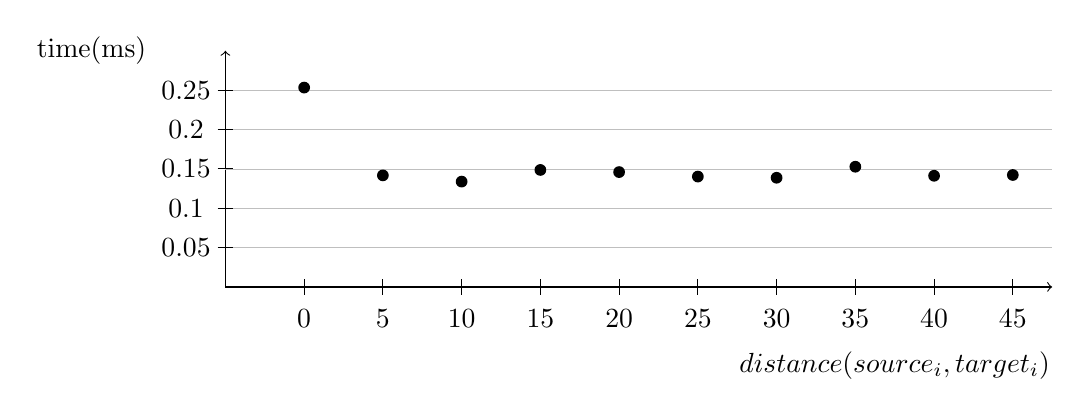
\begin{tikzpicture}[yscale=10]
	%time axis
	\draw[->] (0,0) -- (0,0.3);
	\node at (-1.7, 0.3){time(ms)};
	
	\foreach \y in {0.05, 0.1, 0.15, 0.2, 0.25}{
		\draw[very thin, lightgray] (0, \y)--(10.5, \y);
		\draw(-0.1, \y)--(0.1, \y);
		\node at (-0.5, \y){\y};
		
	}
	
	\draw[->] (0,0) -- (10.5, 0);
	\node at (8.5, -0.1){$distance(source_i, target_{i})$};
	\foreach \x in {0, 1, 2, ..., 9}{
		\draw(\x+1, 0.01)--(\x+1, -0.01);
	}
	\node at (1, -0.04){$0$};
	\node at (2, -0.04){$5$};
	\node at (3, -0.04){$10$};
	\node at (4, -0.04){$15$};
	\node at (5, -0.04){$20$};
	\node at (6, -0.04){$25$};
	\node at (7, -0.04){$30$};
	\node at (8, -0.04){$35$};
	\node at (9, -0.04){$40$};
	\node at (10, -0.04){$45$};
	
	\node at (1, 0.2532) [circle,fill,inner sep=1.5pt]{};
	\node at (2, 0.1417) [circle,fill,inner sep=1.5pt]{};
	\node at (3, 0.1338) [circle,fill,inner sep=1.5pt]{};
	\node at (4, 0.1486) [circle,fill,inner sep=1.5pt]{};
	\node at (5, 0.1459) [circle,fill,inner sep=1.5pt]{};
	\node at (6, 0.1402) [circle,fill,inner sep=1.5pt]{};
	\node at (7, 0.13868) [circle,fill,inner sep=1.5pt]{};
	\node at (8, 0.1527) [circle,fill,inner sep=1.5pt]{};
	\node at (9, 0.1412) [circle,fill,inner sep=1.5pt]{};
	\node at (10, 0.1422) [circle,fill,inner sep=1.5pt]{};
	\end{tikzpicture}
	\centering
	\caption{Average run times of the \textit{OrderConstraint} with a distance between subsequent $source$ events of $11$ in dependency of the distance $source$ events and their associated $target$ event}
	\label{fig:OrderConstraintRunTime2}
\end{figure}

\subsubsection{SporadicConstraint}
The traces, that were used for the fulfill the constraint with the parameters $jitter\in\{1,11,21,31\}$, $lower\in\{500,600,...,900\}$ and $upper=lower+x$ $x\in\{100, 200, ..., 500\}$. The run times were between 0.014ms and 56.26ms, with an average of 0.4ms. The average run time per timestamps of the monitor with the parameters $lower=500$ and $upper=600$ with different values for the $jitter$ parameter can be seen in Figure~\ref{fig:SporadicConstraintRuntime1}. Similar to the run times with varying $upper$ values (figure~\ref{fig:SporadicConstraintRuntime2}), the run times are nearly constant. Like expected by the analysis of the implementation in the previous section, the parameters had no influence on the run time.

\begin{figure}
	\centering
	\begin{minipage}{0.45\textwidth}
		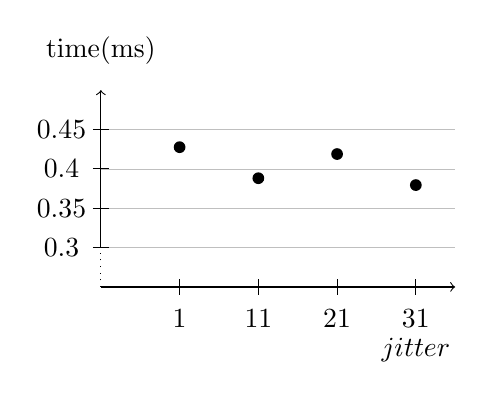
\begin{tikzpicture}[yscale=10]
		%time axis
		\draw[->] (0,0.3) -- (0,0.5);
		\draw[dotted] (0, 0.25) -- (0,0.3);
		\node at (0, 0.55){time(ms)};
		
		\foreach \y in {0.3, 0.35, 0.4, 0.45}{
			\draw[very thin, lightgray] (0, \y)--(4.5, \y);
			\draw(-0.1, \y)--(0.1, \y);
			\node at (-0.5, \y){\y};
		
		}
		
		\draw[->] (0,0.25) -- (4.5, 0.25);
		\node at (4, 0.17){$jitter$};
		\foreach \x in {0, 1, 2, ..., 3}{
			\draw(\x+1, 0.26)--(\x+1, 0.24);
		}
		\node at (1, 0.21){$1$};
		\node at (2, 0.21){$11$};
		\node at (3, 0.21){$21$};
		\node at (4, 0.21){$31$};
		\node at (1, 0.4275) [circle,fill,inner sep=1.5pt]{};
		\node at (2, 0.3881) [circle,fill,inner sep=1.5pt]{};
		\node at (3, 0.4188) [circle,fill,inner sep=1.5pt]{};
		\node at (4, 0.3794) [circle,fill,inner sep=1.5pt]{};
		\end{tikzpicture}
		\centering
		\caption{Average run times of the\\ \textit{SporadicConstraint} with the\\ parameters $lower = 500, upper = 900$}
		\label{fig:SporadicConstraintRuntime1}
	\end{minipage}\hfill
	\begin{minipage}{0.45\textwidth}
		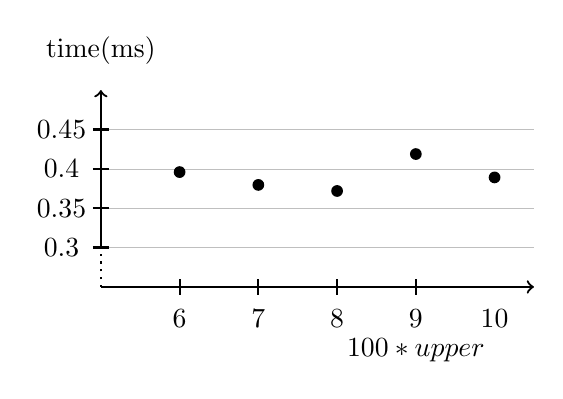
\begin{tikzpicture}[thick, yscale=10]
		%time axis
		\draw[->] (0,0.3) -- (0,0.5);
		\draw[dotted] (0, 0.25) -- (0,0.3);
		\node at (0,0.55){time(ms)};
		
		\foreach \y in {0.3, 0.35, 0.4, 0.45}{
			\draw[very thin, lightgray] (0, \y)--(5.5, \y);
			\draw(-0.1, \y)--(0.1, \y);
			\node at (-0.5, \y){\y};
		
		}
		
		\draw[->] (0,0.25) -- (5.5, 0.25);
		\node at (4, 0.17){$100*upper$};
		\foreach \x in {0, 1, 2, ..., 3}{
			\draw(\x+1, 0.26)--(\x+1, 0.24);
		}
		\node at (1, 0.21){$6$};
		\node at (2, 0.21){$7$};
		\node at (3, 0.21){$8$};
		\node at (4, 0.21){$9$};
		\node at (5, 0.21){$10$};
		\node at (1, 0.3959) [circle,fill,inner sep=1.5pt]{};
		\node at (2, 0.3796) [circle,fill,inner sep=1.5pt]{};
		\node at (3, 0.3719) [circle,fill,inner sep=1.5pt]{};
		\node at (4, 0.4188) [circle,fill,inner sep=1.5pt]{};
		\node at (5, 0.3891) [circle,fill,inner sep=1.5pt]{};
		\end{tikzpicture}
		\centering
		\caption{Average run times of the\\ \textit{SporadicConstraint} with the parameters\\ $lower = 500, jitter = 21$}
		\label{fig:SporadicConstraintRuntime2}
	\end{minipage}
\end{figure}

\subsubsection{PeriodicConstraint}
The run time evaluation was done on traces, which fulfill the \textit{PeriodicConstraint} with the parameters $period\in\{10,20,30,..,100\}$ and $jitter\in\{0,1,..,9\}$. The run time per event was between 0.016ms and 40.39ms, with an average of 0.39ms. In figure~\ref{fig:PeriodicConstrainttRunTime1} the average run times of the monitor with a constant $period$ and a variable $jitter$ can be seen, in figure~\ref{fig:PeriodicConstrainttRunTime2}, $jitter$ is fixed and $period$ is variable. Despite some fluctuations, the run time is constant and independent of the input parameters. This behaviour was expected by the complexity analysis.

\begin{figure}
	\centering
	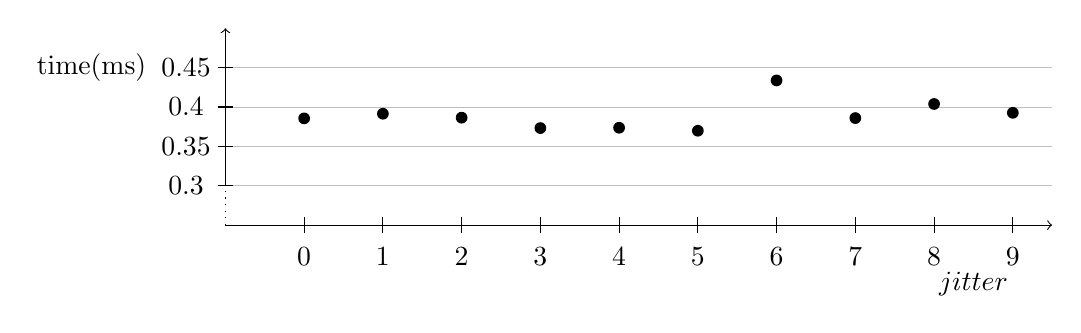
\begin{tikzpicture}[yscale=10]
	%time axis
	\draw[->] (0,0.3) -- (0,0.5);
	\draw[dotted] (0, 0.25) -- (0,0.3);
	\node at (-1.7, 0.45){time(ms)};
	
	\foreach \y in {0.3, 0.35, 0.4, 0.45}{
		\draw[very thin, lightgray] (0, \y)--(10.5, \y);
		\draw(-0.1, \y)--(0.1, \y);
		\node at (-0.5, \y){\y};
	
	}
	
	\draw[->] (0,0.25) -- (10.5, 0.25);
	\node at (9.5, 0.175){$jitter$};
	\foreach \x in {0, 1, 2, ..., 9}{
		\draw(\x+1, 0.26)--(\x+1, 0.24);
		\node at (\x+1, 0.21){$\x$};
	}

	\node at (1, 0.3855) [circle,fill,inner sep=1.5pt]{};
	\node at (2, 0.3914) [circle,fill,inner sep=1.5pt]{};
	\node at (3, 0.3864) [circle,fill,inner sep=1.5pt]{};
	\node at (4, 0.3732) [circle,fill,inner sep=1.5pt]{};
	\node at (5, 0.3736) [circle,fill,inner sep=1.5pt]{};
	\node at (6, 0.3698) [circle,fill,inner sep=1.5pt]{};
	\node at (7, 0.4337) [circle,fill,inner sep=1.5pt]{};
	\node at (8, 0.3859) [circle,fill,inner sep=1.5pt]{};
	\node at (9, 0.4038) [circle,fill,inner sep=1.5pt]{};
	\node at (10, 0.3926) [circle,fill,inner sep=1.5pt]{};
	\end{tikzpicture}
	\centering
	\caption{Average run times of the \textit{PeriodicConstraint} with a $period$ of 10 and variable $jitter$}
	\label{fig:PeriodicConstrainttRunTime1}
\end{figure}

\begin{figure}
	\centering
	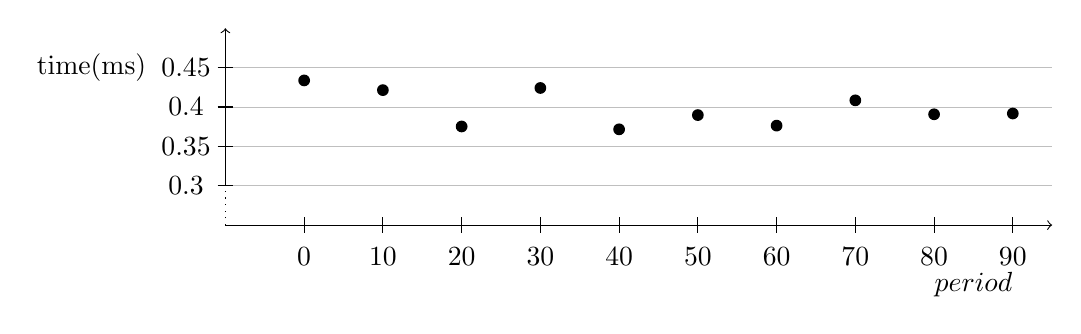
\begin{tikzpicture}[yscale=10]
	%time axis
	\draw[->] (0,0.3) -- (0,0.5);
	\draw[dotted] (0, 0.25) -- (0,0.3);
	\node at (-1.7, 0.45){time(ms)};
	
	\foreach \y in {0.3, 0.35, 0.4, 0.45}{
		\draw[very thin, lightgray] (0, \y)--(10.5, \y);
		\draw(-0.1, \y)--(0.1, \y);
		\node at (-0.5, \y){\y};
	
	}
	
	\draw[->] (0,0.25) -- (10.5, 0.25);
	\node at (9.5, 0.175){$period$};
	\foreach \x in {0, 1, 2, ..., 9}{
		\draw(\x+1, 0.26)--(\x+1, 0.24);
		%\node at (\x+1, 0.21){$\x0$};
	}
	\node at (1, 0.21){$0$};
	\foreach \x in {1, 2, ..., 9}{
		\node at (\x+1, 0.21){$\x0$};
	}
	\node at (1, 0.4337) [circle,fill,inner sep=1.5pt]{};
	\node at (2, 0.4214) [circle,fill,inner sep=1.5pt]{};
	\node at (3, 0.3752) [circle,fill,inner sep=1.5pt]{};
	\node at (4, 0.42413) [circle,fill,inner sep=1.5pt]{};
	\node at (5, 0.3716) [circle,fill,inner sep=1.5pt]{};
	\node at (6, 0.3897) [circle,fill,inner sep=1.5pt]{};
	\node at (7, 0.3763) [circle,fill,inner sep=1.5pt]{};
	\node at (8, 0.4084) [circle,fill,inner sep=1.5pt]{};
	\node at (9, 0.3907) [circle,fill,inner sep=1.5pt]{};
	\node at (10, 0.3917) [circle,fill,inner sep=1.5pt]{};
	\end{tikzpicture}
	\centering
	\caption{Average run times of the \textit{PeriodicConstraint} with a $period$ of 6 and variable $period$}
	\label{fig:PeriodicConstrainttRunTime2}
\end{figure}

\subsubsection{PatternConstraint}
	The monitor of the \emph{PatternConstraint} was first evaluated on traces with lengths of the $|offset|$ parameter of 1, 2 and 3 and varying values for the parameters $period$ and $jitter$. Figure~\ref{fig:PatternConstraintTimeMeasure1} and \ref{fig:PatternConstraintTimeMeasure2} are showing some of these results, which where nearly constant at around 0.65ms per input timestamp. After these run time measurements, the run time was measured on traces with the parameters $jitter=0$ and $period=200$. The $offset$ parameter had an increasing length from 1 to 100 and was filled with $offset=[0, 1, 2, 3, ...]$ and the $period$ parameter was set to 200. The results of this measurement can be seen in figure~\ref{fig:PatternConstraintTimeMeasure3} .It can be seen, that the average run times was nearly constant, beside some measurement deviations. This behaviour was expected by the analysis in the previous section.
	
	\begin{figure}
		\centering
		\begin{minipage}{0.45\textwidth}
			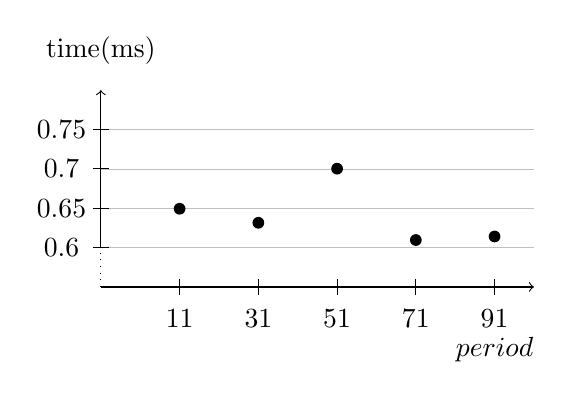
\begin{tikzpicture}[yscale=10]
				%time axis
				\draw[->] (0,0.6) -- (0,0.8);
				\draw[dotted] (0, 0.55) -- (0,0.6);
				\node at (0, 0.85){time(ms)};
				
				\foreach \y in {0.6, 0.65, 0.7, 0.75}{
					\draw[very thin, lightgray] (0, \y)--(5.5, \y);
					\draw(-0.1, \y)--(0.1, \y);
					\node at (-0.5, \y){\y};
				
				}
				
				\draw[->] (0,0.55) -- (5.5, 0.55);
				\node at (5, 0.47){$period$};
				\foreach \x in {0, 1, 2, ..., 3, 4}{
					\draw(\x+1, 0.56)--(\x+1, 0.54);
				}
				\node at (1, 0.51){$11$};
				\node at (2, 0.51){$31$};
				\node at (3, 0.51){$51$};
				\node at (4, 0.51){$71$};
				\node at (5, 0.51){$91$};
				\node at (1, 0.6493) [circle,fill,inner sep=1.5pt]{};
				\node at (2, 0.6315) [circle,fill,inner sep=1.5pt]{};
				\node at (3, 0.7002) [circle,fill,inner sep=1.5pt]{};
				\node at (4, 0.6096) [circle,fill,inner sep=1.5pt]{};
				\node at (5, 0.6141) [circle,fill,inner sep=1.5pt]{};
			\end{tikzpicture}
			\centering
			\caption{Average run times of the\\ \textit{PatternConstraint} with the parameters\\ \textit{offset}$ = [0,1]$ and $jitter = 0$}
			\label{fig:PatternConstraintTimeMeasure1}
		\end{minipage}\hfill
		\begin{minipage}{0.45\textwidth}
			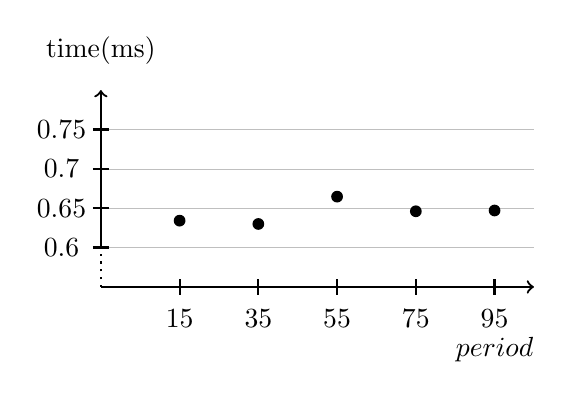
\begin{tikzpicture}[thick, yscale=10]
				%time axis
				\draw[->] (0,0.6) -- (0,0.8);
				\draw[dotted] (0, 0.55) -- (0,0.6);
				\node at (0, 0.85){time(ms)};
				
				\foreach \y in {0.6, 0.65, 0.7, 0.75}{
					\draw[very thin, lightgray] (0, \y)--(5.5, \y);
					\draw(-0.1, \y)--(0.1, \y);
					\node at (-0.5, \y){\y};
					
				}
				
				\draw[->] (0,0.55) -- (5.5, 0.55);
				\node at (5, 0.47){$period$};
				\foreach \x in {0, 1, 2, ..., 3, 4}{
					\draw(\x+1, 0.56)--(\x+1, 0.54);
				}
				\node at (1, 0.51){$15$};
				\node at (2, 0.51){$35$};
				\node at (3, 0.51){$55$};
				\node at (4, 0.51){$75$};
				\node at (5, 0.51){$95$};
				\node at (1, 0.6342) [circle,fill,inner sep=1.5pt]{};
				\node at (2, 0.63) [circle,fill,inner sep=1.5pt]{};
				\node at (3, 0.6647) [circle,fill,inner sep=1.5pt]{};
				\node at (4, 0.6461) [circle,fill,inner sep=1.5pt]{};
				\node at (5, 0.6471) [circle,fill,inner sep=1.5pt]{};
			\end{tikzpicture}
			\centering
			\caption{Average run times of the\\ \textit{PatternConstraint} with the parameters\\ \textit{offset} = $[1,3,5]$ and $jitter = 1$}
			\label{fig:PatternConstraintTimeMeasure2}
		\end{minipage}
	\end{figure}

\begin{figure}
	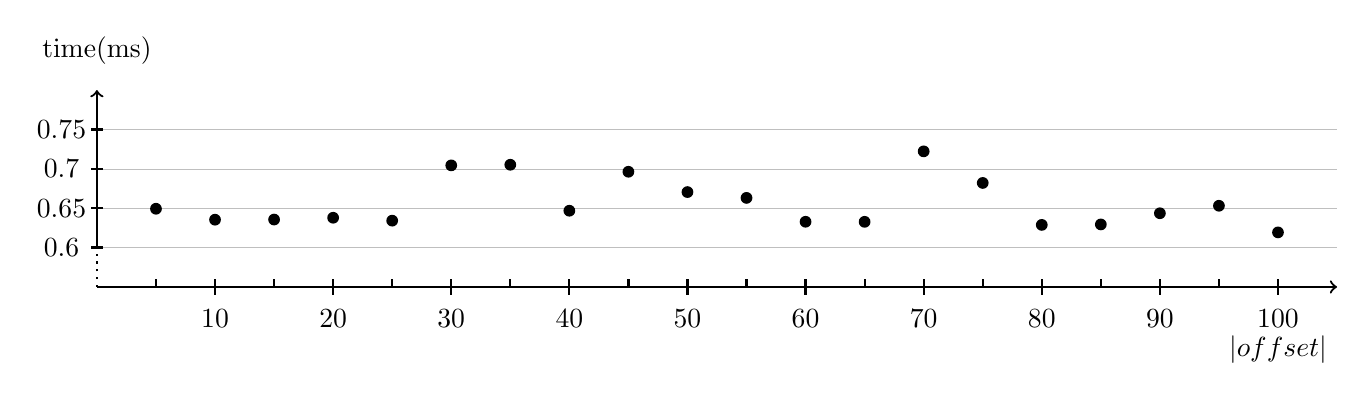
\begin{tikzpicture}[thick, yscale=10, xscale=0.15]
	%time axis
	\draw[->] (0,0.6) -- (0,0.8);
	\draw[dotted] (0, 0.55) -- (0,0.6);
	\node at (0, 0.85){time(ms)};
	
	\foreach \y in { 0.6, 0.65, 0.7, 0.75}{
		\draw[very thin, lightgray] (0, \y)--(105, \y);
		\draw(-0.5, \y)--(0.5, \y);
		\node at (-3, \y){\y};
	}
	
	\draw[->] (0,0.55) -- (105, 0.55);
	\node at (100, 0.47){$|offset|$};
	\foreach \x in {10, 20, ..., 90}{
		\draw(\x, 0.56)--(\x, 0.54);
		\node at (\x, 0.51){$\x$};
		\draw(\x+5, 0.56)--(\x+5, 0.55);
	}
	\draw(100, 0.56)--(100, 0.54);
	\draw(5, 0.56)--(5, 0.55);
	\node at (100, 0.51){100};
	
	\node at (5, 0.6493) [circle,fill,inner sep=1.5pt]{};
	\node at (10, 0.6354) [circle,fill,inner sep=1.5pt]{};
	\node at (15, 0.6356) [circle,fill,inner sep=1.5pt]{};
	\node at (20, 0.6379) [circle,fill,inner sep=1.5pt]{};
	\node at (25, 0.6342) [circle,fill,inner sep=1.5pt]{};
	\node at (30, 0.7044) [circle,fill,inner sep=1.5pt]{};
	\node at (35, 0.7052) [circle,fill,inner sep=1.5pt]{};
	\node at (40, 0.6468) [circle,fill,inner sep=1.5pt]{};
	\node at (45, 0.6963) [circle,fill,inner sep=1.5pt]{};
	\node at (50, 0.6705) [circle,fill,inner sep=1.5pt]{};
	\node at (55, 0.6631) [circle,fill,inner sep=1.5pt]{};
	\node at (60, 0.6328) [circle,fill,inner sep=1.5pt]{};
	\node at (65, 0.6327) [circle,fill,inner sep=1.5pt]{};
	\node at (70, 0.7222) [circle,fill,inner sep=1.5pt]{};
	\node at (75, 0.6821) [circle,fill,inner sep=1.5pt]{};
	\node at (80, 0.6288) [circle,fill,inner sep=1.5pt]{};
	\node at (85, 0.6294) [circle,fill,inner sep=1.5pt]{};
	\node at (90, 0.6436) [circle,fill,inner sep=1.5pt]{};
	\node at (95, 0.6531) [circle,fill,inner sep=1.5pt]{};
	\node at (100, 0.6193) [circle,fill,inner sep=1.5pt]{};

	\end{tikzpicture}
	\centering
	\caption{Average run times of the \textit{PatternConstraint} with the parameters \textit{period} $= 200$ and $jitter = 0$}
	\label{fig:PatternConstraintTimeMeasure3}
\end{figure}


\subsubsection{ArbitraryConstraint}
	% TODO größere Unterschiede in minimum länge
	Similar to the previous constraint, multiple runs were done for the run time measurement. First with small lengths of the $minimum$ and $maximum$ parameter and changing values for the values inside of these parameters, and then with a length of the $minimum$ and $maximum$ parameter of 1 to 100. Figure~\ref{fig:ArbitraryConstraintTimeMeasure1} and \ref{fig:ArbitraryConstraintTimeMeasure2} are showing some of the results with short $minimum$ and $maximum$ parameters. It can be seen, that the results with the same length of these parameters are nearly constant, but the traces with a $minimum$ length of 3 took slightly slightly more time.%TODO langes minimum
	\begin{figure}
	\centering
	\begin{minipage}{0.45\textwidth}
		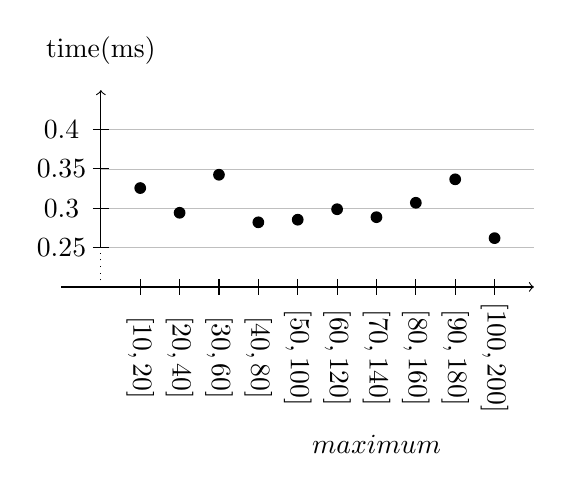
\begin{tikzpicture}[yscale=10]
		%time axis
		\draw[->] (0.5,0.25) -- (0.5,0.45);
		\draw[dotted] (0.5, 0.2) -- (0.5,0.25);
		\node at (0.5, 0.5){time(ms)};
		
		\foreach \y in {0.25, 0.3, 0.35, 0.4}{
			\draw[very thin, lightgray] (0.5, \y)--(6, \y);
			\draw(0.4, \y)--(0.6, \y);
			\node at (0, \y){\y};
			
		}
		
		\draw[->] (0,0.2) -- (6, 0.2);
		\node at (4, 0.0){$maximum$};
		\foreach \x in {0, 0.5, 1, ..., 4.5}{
			\draw(\x+1, 0.21)--(\x+1, 0.19);
		}
		\node[rotate=270] at (1, 0.11){$[10,20]$};
		\node[rotate=270] at (1.5, 0.11){$[20,40]$};
		\node[rotate=270] at (2, 0.11){$[30,60]$};
		\node[rotate=270] at (2.5, 0.11){$[40,80]$};
		\node[rotate=270] at (3, 0.11){$[50,100]$};
		\node[rotate=270] at (3.5, 0.11){$[60,120]$};
		\node[rotate=270] at (4, 0.11){$[70,140]$};
		\node[rotate=270] at (4.5, 0.11){$[80,160]$};
		\node[rotate=270] at (5, 0.11){$[90,180]$};
		\node[rotate=270] at (5.5, 0.11){$[100,200]$};
		\node at (1, 0.3256) [circle,fill,inner sep=1.5pt]{};
		\node at (1.5, 0.2942) [circle,fill,inner sep=1.5pt]{};
		\node at (2, 0.3425) [circle,fill,inner sep=1.5pt]{};
		\node at (2.5, 0.2821) [circle,fill,inner sep=1.5pt]{};
		\node at (3, 0.2854) [circle,fill,inner sep=1.5pt]{};
		\node at (3.5, 0.2987) [circle,fill,inner sep=1.5pt]{};
		\node at (4, 0.2886) [circle,fill,inner sep=1.5pt]{};
		\node at (4.5, 0.3069) [circle,fill,inner sep=1.5pt]{};
		\node at (5, 0.3367) [circle,fill,inner sep=1.5pt]{};
		\node at (5.5, 0.262) [circle,fill,inner sep=1.5pt]{};
		\end{tikzpicture}
		\centering
		\caption{Average run times of the\\ \textit{ArbitraryConstraint} with the\\ parameter $minimum = [10,20]$}
		\label{fig:ArbitraryConstraintTimeMeasure1}
	\end{minipage}\hfill
	\begin{minipage}{0.45\textwidth}
		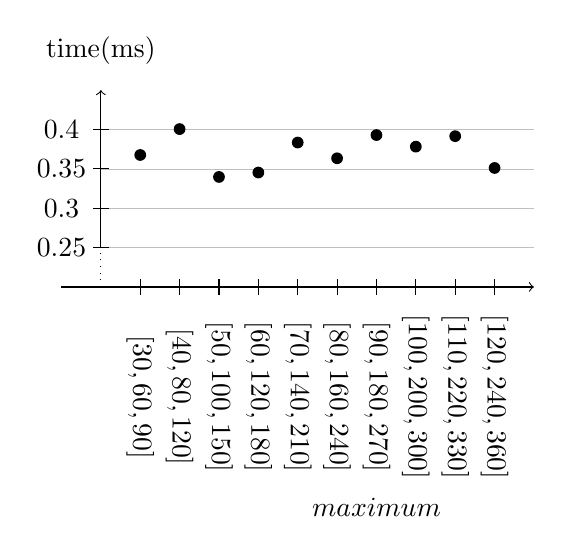
\begin{tikzpicture}[yscale=10]
		%time axis
			\draw[->] (0.5,0.25) -- (0.5,0.45);
			\draw[dotted] (0.5, 0.2) -- (0.5,0.25);
			\node at (0.5, 0.5){time(ms)};
			
			\foreach \y in {0.25, 0.3, 0.35, 0.4}{
				\draw[very thin, lightgray] (0.5, \y)--(6, \y);
				\draw(0.4, \y)--(0.6, \y);
				\node at (0, \y){\y};
				
			}
			
			\draw[->] (0,0.2) -- (6, 0.2);
			\node at (4, -0.08){$maximum$};
			\foreach \x in {0, 0.5, 1, ..., 4.5}{
				\draw(\x+1, 0.21)--(\x+1, 0.19);
			}
			\node[rotate=270] at (1, 0.06)	{$[30 ,60 ,90]$};
			\node[rotate=270] at (1.5, 0.06){$[40 ,80 ,120]$};
			\node[rotate=270] at (2, 0.06)	{$[50 ,100,150]$};
			\node[rotate=270] at (2.5, 0.06){$[60 ,120,180]$};
			\node[rotate=270] at (3, 0.06)	{$[70 ,140,210]$};
			\node[rotate=270] at (3.5, 0.06){$[80 ,160,240]$};
			\node[rotate=270] at (4, 0.06)	{$[90 ,180,270]$};
			\node[rotate=270] at (4.5, 0.06){$[100,200,300]$};
			\node[rotate=270] at (5, 0.06)	{$[110,220,330]$};
			\node[rotate=270] at (5.5, 0.06){$[120,240,360]$};
			\node at (1, 0.3676) [circle,fill,inner sep=1.5pt]{};
			\node at (1.5, 0.4005) [circle,fill,inner sep=1.5pt]{};
			\node at (2, 0.3397) [circle,fill,inner sep=1.5pt]{};
			\node at (2.5, 0.3453) [circle,fill,inner sep=1.5pt]{};
			\node at (3, 0.3834) [circle,fill,inner sep=1.5pt]{};
			\node at (3.5, 0.3634) [circle,fill,inner sep=1.5pt]{};
			\node at (4, 0.3929) [circle,fill,inner sep=1.5pt]{};
			\node at (4.5, 0.3782) [circle,fill,inner sep=1.5pt]{};
			\node at (5, 0.3915) [circle,fill,inner sep=1.5pt]{};
			\node at (5.5, 0.3511) [circle,fill,inner sep=1.5pt]{};
		\end{tikzpicture}
		\centering
		\caption{Average run times of the\\ \textit{ArbitraryConstraint} with the\\ parameter $minimum = [30,60, 90]$}
		\label{fig:ArbitraryConstraintTimeMeasure2}
	\end{minipage}
\end{figure}
	

\subsubsection{BurstConstraint}
	Figure~\ref{fig:BurstConstraintRunTime} shows the average run time per input timestamp in with increasing a number of occurrences per burst. Similar to the \textit{RepeatConstraint}, over which the \textit{BurstConstraint} is defined and implemented, are small increase in the run times can be seen by increasing the number of occurrences. This increase is smaller than the fluctuations between the individual measurements, but the trend can be seen in all of the results. The linear growth was expected by the analysis in the previous section.
\begin{figure}
	\centering
	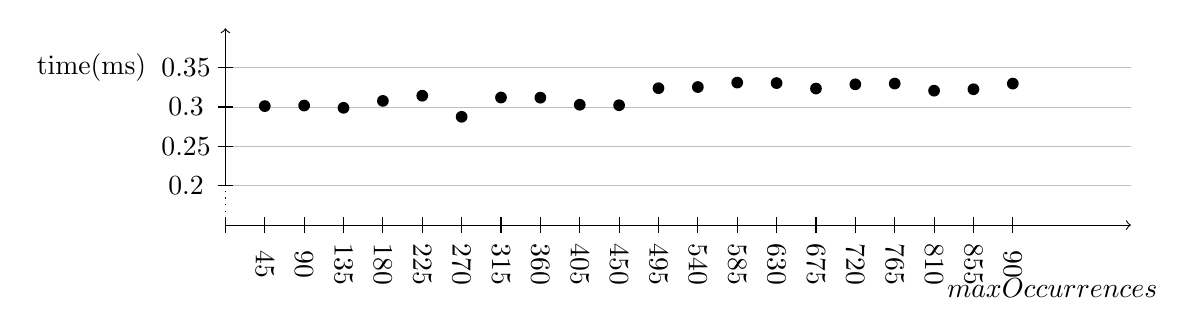
\begin{tikzpicture}[yscale=10]
	%time axis
	\draw[->] (0,0.2) -- (0,0.4);
	\draw[dotted] (0, 0.15) -- (0,0.2);
	\node at (-1.7, 0.35){time(ms)};
	
	\foreach \y in {0.2, 0.25, 0.3, 0.35}{
		\draw[very thin, lightgray] (0, \y)--(11.5, \y);
		\draw(-0.1, \y)--(0.1, \y);
		\node at (-0.5, \y){\y};
		
	}
	
	\draw[->] (0,0.15) -- (11.5, 0.15);
	\node at (10.5, 0.07){$maxOccurrences$};
	\foreach \x in {0, 1, 2, ..., 9}{
		\draw(\x, 0.16)--(\x, 0.14);
		\draw(\x+0.5, 0.16)--(\x+0.5, 0.14);
		%\node at (\x+1, 0.21){$\x0$};
	}
	\draw(10, 0.16)--(10, 0.14);

	\node[rotate=270] at (0.5, 0.1){$45$};
	\node[rotate=270] at (1, 0.1){$90$};
	\node[rotate=270] at (1.5, 0.1){$135$};
	\node[rotate=270] at (2, 0.1){$180$};
	\node[rotate=270] at (2.5, 0.1){$225$};
	\node[rotate=270] at (3, 0.1){$270$};
	\node[rotate=270] at (3.5, 0.1){$315$};
	\node[rotate=270] at (4, 0.1){$360$};
	\node[rotate=270] at (4.5, 0.1){$405$};
	\node[rotate=270] at (5, 0.1){$450$};
	\node[rotate=270] at (5.5, 0.1){$495$};
	\node[rotate=270] at (6, 0.1){$540$};
	\node[rotate=270] at (6.5, 0.1){$585$};
	\node[rotate=270] at (7, 0.1){$630$};
	\node[rotate=270] at (7.5, 0.1){$675$};
	\node[rotate=270] at (8, 0.1){$720$};
	\node[rotate=270] at (8.5, 0.1){$765$};
	\node[rotate=270] at (9, 0.1){$810$};
	\node[rotate=270] at (9.5, 0.1){$855$};
	\node[rotate=270] at (10, 0.1){$90$};

	\node at (0.5, 0.3011) [circle,fill,inner sep=1.5pt]{};
	\node at (1, 0.3018) [circle,fill,inner sep=1.5pt]{};
	\node at (1.5, 0.2989) [circle,fill,inner sep=1.5pt]{};
	\node at (2, 0.3077) [circle,fill,inner sep=1.5pt]{};
	\node at (2.5, 0.3143) [circle,fill,inner sep=1.5pt]{};
	\node at (3, 0.2875) [circle,fill,inner sep=1.5pt]{};
	\node at (3.5, 0.312) [circle,fill,inner sep=1.5pt]{};
	\node at (4, 0.3118) [circle,fill,inner sep=1.5pt]{};
	\node at (4.5, 0.3028) [circle,fill,inner sep=1.5pt]{};
	\node at (5, 0.3022) [circle,fill,inner sep=1.5pt]{};
	\node at (5.5, 0.3238) [circle,fill,inner sep=1.5pt]{};
	\node at (6, 0.3253) [circle,fill,inner sep=1.5pt]{};
	\node at (6.5, 0.330935) [circle,fill,inner sep=1.5pt]{};
	\node at (7, 0.330328) [circle,fill,inner sep=1.5pt]{};
	\node at (7.5, 0.323373) [circle,fill,inner sep=1.5pt]{};
	\node at (8, 0.328733) [circle,fill,inner sep=1.5pt]{};
	\node at (8.5, 0.329728) [circle,fill,inner sep=1.5pt]{};
	\node at (9, 0.320669) [circle,fill,inner sep=1.5pt]{};
	\node at (9.5, 0.322486) [circle,fill,inner sep=1.5pt]{};
	\node at (10, 0.329673) [circle,fill,inner sep=1.5pt]{};
	\end{tikzpicture}
	\centering
	\caption{Average run times of the \textit{BurstConstraint} with increasing $occurrences$ per burst}
	\label{fig:BurstConstraintRunTime}
\end{figure}

\subsubsection{ReactionConstraint}
The runtime evaluation of the \textit{ReactionConstraint} was done on traces with the parameters $minimum\in\{100,200,...,1000\}$ and $maximum = minimum$, while the distances between subsequent $stimulus$ event were in $\{1, 2, 4, 8, ..., 1024\}$, so that $minimum$, $\lceil\frac{minimum}{2}\rceil$,  $\lceil\frac{minimum}{4}\rceil$, ...,  $\lceil\frac{minimum}{1024}\rceil$ events must be stored and considered at every event in the monitor. The runtime per event was between 0.15ms and 42.36ms, with an average of 2ms. Figure~\ref{fig:ReactionConstraintRunTime1} and \ref{fig:ReactionConstraintRunTime2} are showing the average run times of the monitor with increasing $minimum$ and $maximum$ parameters, but fixed distance between subsequent $stimulus$ events. The first figure shows the run times with $stimulus$ distances of 1, which is the worst case, because $maximum$ events must be stored and considered for the correctness decision of the monitor. Like expected by the analysis, the run time is increasing linear with larger $maximum$ values. This behaviour can also be seen in the second figure, where the distance between the events is 128, but the run times are much smaller here. This is, because between 1 ($\lceil \frac{100}{128}\rceil$) and 8 ($\lceil \frac{1000}{128}\rceil$) were considered in each timestamp with events, not between 100 and 1000 in the previous case.
\begin{figure}
	\centering
	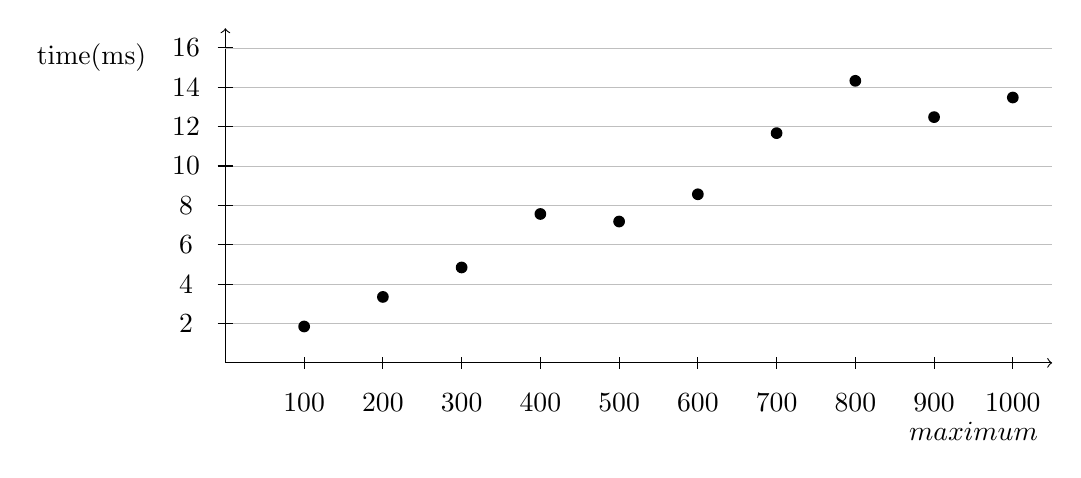
\begin{tikzpicture}[yscale=0.25]
	%time axis
	\draw[->] (0,0) -- (0,17);
	\node at (-1.7, 15.5){time(ms)};
	
	\foreach \y in {2, 4, ..., 16}{
		\draw[very thin, lightgray] (0, \y)--(10.5, \y);
		\draw(-0.1, \y)--(0.1, \y);
		\node at (-0.5, \y){\y};
		
	}
	
	\draw[->] (0,0) -- (10.5, 0.0);
	\node at (9.5, -3.5){$maximum$};
	\foreach \x in {1, 2, ..., 9, 10}{
		\draw(\x, -0.3)--(\x, 0.3);
		\node at (\x, -2){$\x00$};
	}
	\node at (1, 1.8486) [circle,fill,inner sep=1.5pt]{};
	\node at (2, 3.3500) [circle,fill,inner sep=1.5pt]{};
	\node at (3, 4.8465) [circle,fill,inner sep=1.5pt]{};
	\node at (4, 7.5645) [circle,fill,inner sep=1.5pt]{};
	\node at (5, 7.1811) [circle,fill,inner sep=1.5pt]{};
	\node at (6, 8.5639) [circle,fill,inner sep=1.5pt]{};
	\node at (7, 11.6705) [circle,fill,inner sep=1.5pt]{};
	\node at (8, 14.3276) [circle,fill,inner sep=1.5pt]{};
	\node at (9, 12.4841) [circle,fill,inner sep=1.5pt]{};
	\node at (10, 13.4801) [circle,fill,inner sep=1.5pt]{};
	\end{tikzpicture}
	\centering
	\caption{Average run times of the \textit{ReactionConstraint} with a distance between subsequent $stimulus$ events of 1 (worst case)  and variable $maximum$}
	\label{fig:ReactionConstraintRunTime1}
\end{figure}

\begin{figure}
	\centering
	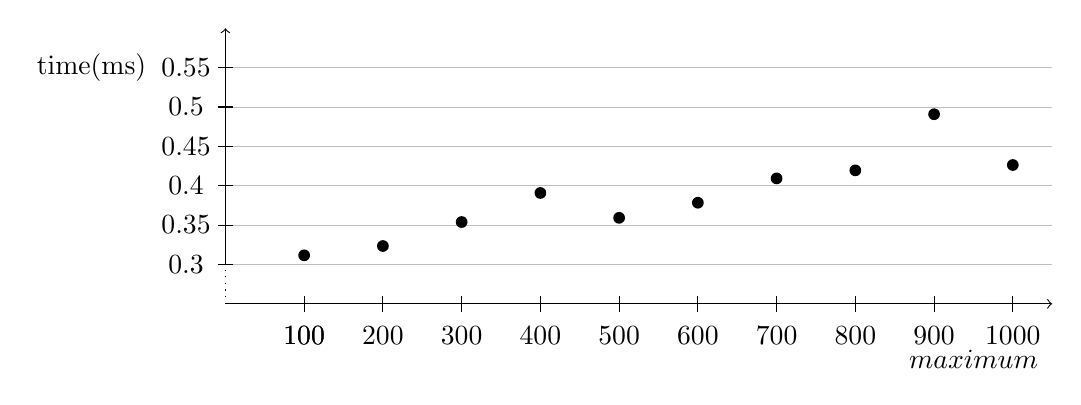
\begin{tikzpicture}[yscale=10]
		\draw[->] (0,0.3) -- (0,0.6);
		\draw[dotted] (0, 0.25) -- (0,0.3);
		\node at (-1.7, 0.55){time(ms)};
		
		\foreach \y in {0.3, 0.35, 0.4, 0.45, 0.5, 0.55}{
			\draw[very thin, lightgray] (0, \y)--(10.5, \y);
			\draw(-0.1, \y)--(0.1, \y);
			\node at (-0.5, \y){\y};
			
		}
		
		\draw[->] (0,0.25) -- (10.5, 0.25);
		\node at (9.5, 0.18){$maximum$};
		\foreach \x in {1, 1, 2, ..., 10}{
			\draw(\x, 0.26)--(\x, 0.24);
			\node at (\x, 0.21){$\x00$};
		}
		\node at (1, 0.3116) [ circle,fill,inner sep=1.5pt]{};
		\node at (2, 0.3234) [ circle,fill,inner sep=1.5pt]{};
		\node at (3, 0.3539) [ circle,fill,inner sep=1.5pt]{};
		\node at (4, 0.3908) [ circle,fill,inner sep=1.5pt]{};
		\node at (5, 0.3592) [ circle,fill,inner sep=1.5pt]{};
		\node at (6, 0.3784) [ circle,fill,inner sep=1.5pt]{};
		\node at (7, 0.4093) [ circle,fill,inner sep=1.5pt]{};
		\node at (8, 0.4195) [ circle,fill,inner sep=1.5pt]{};
		\node at (9, 0.4908) [ circle,fill,inner sep=1.5pt]{};
		\node at (10, 0.4263) [ circle,fill,inner sep=1.5pt]{};
	\end{tikzpicture}
	\centering
	\caption{Average run times of the \textit{ReactionConstraint} with a distance between subsequent $stimulus$ events of 128 and variable $maximum$}
	\label{fig:ReactionConstraintRunTime2}
\end{figure}

\subsubsection{AgeConstraint}
The run time of the \textit{AgeConstraint} monitor were measured on traces with the same parameters as the previous constraint. Figure~\ref{fig:AgeConstraintRunTime1} shows the run times with event distances of 1, which is the worst case in terms of monitoring, in dependency of the $maximum$ parameter. With increasing $maximum$ values, the average run time grew linear, like expected in the analysis. The average run times with the same $maximum$ values and a distance between subsequent $stimulus$ events is shown in figure~\ref{fig:AgeConstraintRunTime2}. The run time is growing nearly linear again. Deviations can be seen at $maximum=500$ and $maximum=1000$. Because $\lceil\frac{400}{128}\rceil=\lceil\frac{500}{128}\rceil$ and $\lceil\frac{900}{128}\rceil=\lceil\frac{1000}{128}\rceil$, the number of events, which must be stored, and considered in each input timestamp. Therefore, the run time is not increasing at these parameter values.
\begin{figure}
	\centering
	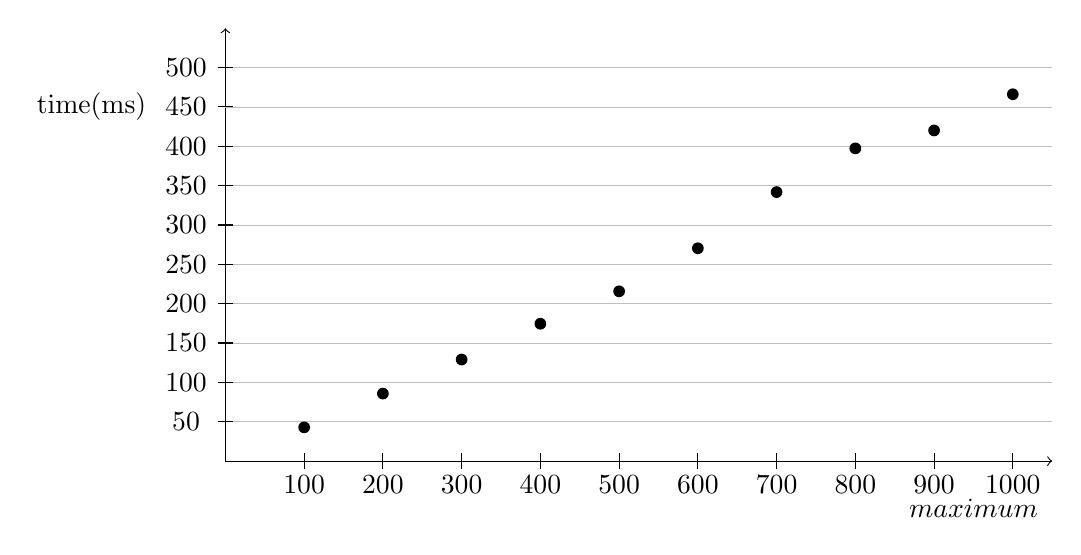
\begin{tikzpicture}[yscale=0.01]
	%time axis
	\draw[->] (0,0) -- (0,550);
	\node at (-1.7, 450){time(ms)};
	
	\foreach \y in {50, 100, ..., 500}{
		\draw[very thin, lightgray] (0, \y)--(10.5, \y);
		\draw(-0.1, \y)--(0.1, \y);
		\node at (-0.5, \y){\y};
		
	}
	
	\draw[->] (0,0) -- (10.5, 0.0);
	\node at (9.5, -60){$maximum$};
	\foreach \x in {1, 2, ..., 9, 10}{
		\draw(\x, -10)--(\x, 10);
		\node at (\x, -30){$\x00$};
	}
	\node at (1, 42.82) [circle,fill,inner sep=1.5pt]{};
	\node at (2, 85.72) [circle,fill,inner sep=1.5pt]{};
	\node at (3, 129.0) [circle,fill,inner sep=1.5pt]{};
	\node at (4, 174.49) [circle,fill,inner sep=1.5pt]{};
	\node at (5, 215.69) [circle,fill,inner sep=1.5pt]{};
	\node at (6, 270.4) [circle,fill,inner sep=1.5pt]{};
	\node at (7, 341.8) [circle,fill,inner sep=1.5pt]{};
	\node at (8, 397.33) [circle,fill,inner sep=1.5pt]{};
	\node at (9, 420.1) [circle,fill,inner sep=1.5pt]{};
	\node at (10, 466.1) [circle,fill,inner sep=1.5pt]{};
	\end{tikzpicture}
	\centering
	\caption{Average run times of the \textit{AgeConstraint} with a distance between subsequent $stimulus$ events of 1 (worst case)  and variable $maximum$}
	\label{fig:AgeConstraintRunTime1}
\end{figure}

\begin{figure}
	\centering
	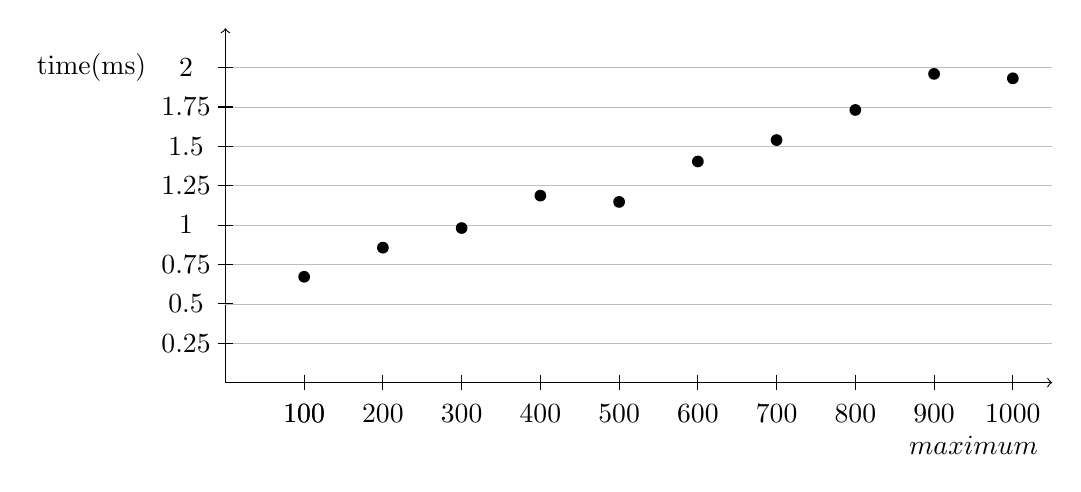
\begin{tikzpicture}[yscale=2]
	\draw[->] (0,0) -- (0,2.25);
	\node at (-1.7, 2){time(ms)};
	
	\foreach \y in {0.25, 0.5, 0.75, 1, 1.25, 1.5, 1.75, 2}{
		\draw[very thin, lightgray] (0, \y)--(10.5, \y);
		\draw(-0.1, \y)--(0.1, \y);
		\node at (-0.5, \y){\y};
		
	}
	
	\draw[->] (0,0) -- (10.5, 0);
	\node at (9.5, -0.4){$maximum$};
	\foreach \x in {1, 1, 2, ..., 10}{
		\draw(\x, 0.05)--(\x, -0.05);
		\node at (\x, -0.2){$\x00$};
	}
	\node at (1, 0.6717) [ circle,fill,inner sep=1.5pt]{};
	\node at (2, 0.8566) [ circle,fill,inner sep=1.5pt]{};
	\node at (3, 0.9811) [ circle,fill,inner sep=1.5pt]{};
	\node at (4, 1.187) [ circle,fill,inner sep=1.5pt]{};
	\node at (5, 1.147) [ circle,fill,inner sep=1.5pt]{};
	\node at (6, 1.404) [ circle,fill,inner sep=1.5pt]{};
	\node at (7, 1.5398) [ circle,fill,inner sep=1.5pt]{};
	\node at (8, 1.731) [ circle,fill,inner sep=1.5pt]{};
	\node at (9, 1.96) [ circle,fill,inner sep=1.5pt]{};
	\node at (10, 1.932) [ circle,fill,inner sep=1.5pt]{};
	\end{tikzpicture}
	\centering
	\caption{Average run times of the \textit{AgeConstraint} with a distance between subsequent $stimulus$ events of 128 and variable $maximum$}
	\label{fig:AgeConstraintRunTime2}
\end{figure}

\subsubsection{OutputSynchronizationConstraint}
%TODO Laufzeit nimmt zu


\subsubsection{InputSynchronizationConstraint}
The traces for the evaluation of the \textit{InputSynchronizationConstraint} were generated with 2,3, 4 and 5 $stimulus$ streams, $tolerance$ values of 10 to 25 in steps of 3 and a distance between synchronization clusters of 2, 4, 8, 16 or 32.\\ Figure~\ref{fig:InputSynchronizationConstraintRuntime1} shows the run time of the monitor with the traces with three $stimulus$ streams and a fix cluster distance of 2. The run times are nearly constant, which was expected by the analysis of the source code. Figure~\ref{fig:InputSynchronizationConstraintRuntime2} shows the average run time with a fixed cluster distance and $tolerance$. It can be see, that the run time increases more than linear with a larger number of input streams, which matches with the analysis, where the run time was expected to grow by the square of $|stimulus|$.

\begin{figure}
	\centering
	\begin{minipage}{0.45\textwidth}
		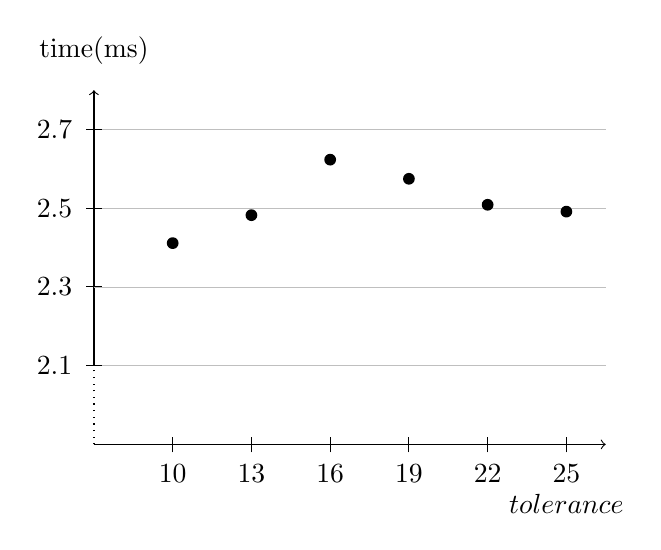
\begin{tikzpicture}[yscale=5]
		%time axis
		\draw[->] (0,2.1) -- (0,2.8);
		\draw[dotted] (0, 1.9) -- (0,2.1);
		\node at (0, 2.9){time(ms)};
		
		\foreach \y in {2.1, 2.3, 2.5 , 2.7}{
			\draw[very thin, lightgray] (0, \y)--(6.5, \y);
			\draw(-0.1, \y)--(0.1, \y);
			\node at (-0.5, \y){\y};
			
		}
		
		\draw[->] (0,1.9) -- (6.5, 1.9);
		\node at (6, 1.75){$tolerance$};
		\foreach \x in {0, 1, 2, ..., 5}{
			\draw(\x+1, 1.88)--(\x+1, 1.92);
		}
		\node at (1, 1.825){$10$};
		\node at (2, 1.825){$13$};
		\node at (3, 1.825){$16$};
		\node at (4, 1.825){$19$};
		\node at (5, 1.825){$22$};
		\node at (6, 1.825){$25$};
		\node at (1, 2.4113) [circle,fill,inner sep=1.5pt]{};
		\node at (2, 2.4823) [circle,fill,inner sep=1.5pt]{};
		\node at (3, 2.6233) [circle,fill,inner sep=1.5pt]{};
		\node at (4, 2.5747) [circle,fill,inner sep=1.5pt]{};
		\node at (5, 2.5087) [circle,fill,inner sep=1.5pt]{};
		\node at (6, 2.4913) [circle,fill,inner sep=1.5pt]{};
		\end{tikzpicture}
		\centering
		\caption{Average run times of the\\ \textit{InputSynchronizationConstraint} with 3\\ stimulus streams and a cluster distance of 2}
		\label{fig:InputSynchronizationConstraintRuntime1}
	\end{minipage}\hfill
		\begin{minipage}{0.45\textwidth}
			\begin{tikzpicture}[yscale=0.75]
				%time axis
				\draw[->] (0,0) -- (0,7);
				\node at (0, 7.5){time(ms)};
				
				\foreach \y in {2, 4, 6}{
					\draw[very thin, lightgray] (0, \y)--(4.5, \y);
					\draw(-0.1, \y)--(0.1, \y);
					\node at (-0.5, \y){\y};
					
				}
				
				\draw[->] (0,0) -- (4.5, 0);
				\node at (4, -1){$|stimulus|$};
				\foreach \x in {1,2,3,4}{
					\draw(\x, -0.15)--(\x, 0.15);
				}
				\node at (1, -0.5){$2$};
				\node at (2, -0.5){$3$};
				\node at (3, -0.5){$4$};
				\node at (4, -0.5){$5$};
				\node at (1, 1.571) [circle,fill,inner sep=1.5pt]{};
				\node at (2, 2.663) [circle,fill,inner sep=1.5pt]{};
				\node at (3, 4.495) [circle,fill,inner sep=1.5pt]{};
				\node at (4, 6.67885) [circle,fill,inner sep=1.5pt]{};
			\end{tikzpicture}
			\centering
			\caption{Average run times of the\\ \textit{InputSynchronizationConstraint} with a cluster\\ distance of 8 and $tolerance=16$}
			\label{fig:InputSynchronizationConstraintRuntime2}
	\end{minipage}\hfill
\end{figure}

\begin{figure}

\end{figure}